\documentclass[12pt,a4paper]{article}
\usepackage[utf8]{inputenc}  % important for correct displayment of Umlaute (must appear before \title command!)
\usepackage[T1]{fontenc}
\title{
    \begin{Huge}
        Modellierung chemisch-reagierender Strömungen
    \end{Huge}
    \\[1cm]
    \begin{Large}
        Belegarbeit: Eindimensionale Laminare nicht vorgemischte Flammen
    \end{Large}
    \\[5cm]
}
\author{Maximilian Knespel}

%\documentclass[hausschrift]{TUBAFarbeiten}
%%\usepackage[T1]{fontenc}
%\usepackage[utf8]{inputenc}  % important for correct displayment of Umlaute (must appear before \title command!)
%\TUBAFTitel{Modellierung chemisch-reagierender Strömungen - Belegarbeit: 1D Diffusionsflammen}
%\TUBAFAutor[M.Knespel]{Maximilian Knespel}

\usepackage[parfill]{parskip} % adds a bit of spacing after each paragraph
% not sure why this package is better than \setlength{\parskip}{10pt plus 1pt minus 1pt}
% http://tex.stackexchange.com/questions/74170/have-new-line-between-paragraphs-no-indentation
% http://ctan.org/pkg/parskip
\input{mk_definitions.tex}

\usepackage[backend=bibtex,style=numeric]{biblatex} % ist default style=numeric, % sudo apt-get install biblatex
\usepackage{bibgerm}                  % sudo apt-get install texlive-lang-german
\addbibresource{literatur.bib}


\usepackage{tikz}
\usepackage{pgf}
\usetikzlibrary{arrows,automata}
\usetikzlibrary{positioning}

\tikzset{
    box/.style={ rectangle, draw=black, very thick, minimum height=2em,
                 inner sep=2pt, text centered }
}

\usepackage[
%nonumberlist,   % keine Seitenzahlen anzeigen
toc,             % Einträge im Inhaltsverzeichnis
%,hyperfirst    % only add link to first usage
%,notree, nosuper, nolist % reduces overhead by excluding styles
%nogroupskip%=true % no line skip after single letter group
style=long3col % 3 columns of fixed width (symbol, description, pages)
]
{glossaries}
%Ein eigenes Symbolverzeichnis erstellen
\newglossary[slg]{symbols}{syi}{syg}{Symbolverzeichnis}
\newglossary[slg]{acronyms}{syi}{syg}{Abkürzungen}
%\makeglossaries
\makenoidxglossaries
\loadglsentries[symbols]{beleg-symbols.tex}
\loadglsentries[acronyms]{beleg-acronyms.tex}

% Token not allowed in a PDF string (PDFDocEncoding): removing `math shift'
% http://tex.stackexchange.com/questions/53513/hyperref-token-not-allowed
% => use \ensuremath{$\lambda_2$}{lambda_2}

% The option "hypcap=true" will be ignored for this(caption)
% http://www.mrunix.de/forums/showthread.php?65435-Seltsame-Warnung-bei-Hyperref-Hypercap
% http://tex.stackexchange.com/questions/32344/issue-with-capt-of-package
% => use \captionsetup{type=figure} % or type=table,...

\addto\extrasngerman{\def\figureautorefname{Abb.}} % for use with autoref
\addto\extrasngerman{\def\equationautorefname{Gl.}} 
\addto\extrasngerman{\def\sectionautorefname{Kapitel}} 
\addto\extrasngerman{\def\subsectionautorefname{Kapitel}} 
\addto\extrasngerman{\def\subsubsectionautorefname{Kapitel}} 

%%%%%%%%%%%%%%%%%%%%%%%%%%%%%%%%%%%%%%%%%%%%%%%%%%%%%%%%%%%%%%%%%



\begin{document}

\maketitle
\newpage
\tableofcontents
\newpage

\glsaddall	% adds all defined, even unused, symbols to symbol list
\setglossarystyle{long3col}
\setlength{\glsdescwidth}{0.6\linewidth}
\setlength{\glspagelistwidth}{0.2\linewidth}
\renewcommand*{\glsgroupskip}{}
\printnoidxglossary[type=symbols]
\newpage
\printnoidxglossary[type=acronyms]
%\printnoidxglossaries
\newpage


%%%%%%%%%%%%%%%%%%%%%%%%%%%%%%%%%%%%%%%%%%%%%%%%%%%%%%%%%%%%%%%%%
\section{Aufgabenstellung}
%%%%%%%%%%%%%%%%%%%%%%%%%%%%%%%%%%%%%%%%%%%%%%%%%%%%%%%%%%%%%%%%%
Der Vollständigkeit wegen wird hier noch einmal in eigenen Worten die Aufgabenstellung wiedergegeben.\\

Betrachtet wird eine Methan-Luft-Diffusionsflamme. Der Versuchsaufbau besteht aus zwei gegeneinander gerichteten Einlässen. Gravitationseffekte werden vernachlässigt, sodass ohne Beschränkung der Allgemeinheit Luft als von oben anströmend angenommen werden kann, siehe \autoref{fig:stream}
\begin{figure}[H]
    \begin{center}
        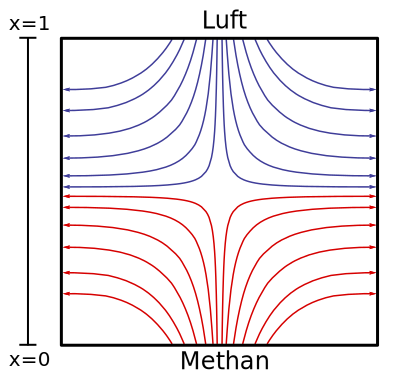
\includegraphics[width=0.4\linewidth]{stream}
    \end{center}
    \caption{Zu simulierender Versuchsaufbau mit qualitativ eingezeichneten Strömungsfeld}
    \label{fig:stream}
\end{figure}

Mit Hilfe des am Institut für Numerische Thermofluiddynamik (\gls{NTFD}) der Technischen Universität Bergakademie Freiberg (\gls{TUBAF}) entwickelten universellen laminaren Flammenlösers (\gls{ULF}) soll der Versuchsaufbau aus \autoref{fig:stream} simuliert und die Ergebnisse ausgewertet werden. Dabei sollen zwei verschiedene Lösungsmethoden angewandt werden: Eine Lösung im physikalischen Raum, also über den Ort diskretisiert und eine Lösung mittels Flamelets.

\begin{sloppypar} % to better break \lstinline (allows larger word distances
\begin{enumerate}
    \item Für die Simulation im physikalischen Raum soll das mit \gls{ULF} mitgelieferte Beispielsetup \lstinline!oppdifJet! benutzt werden. Für diese Konfiguration sind folgende Dinge durchzuführen
    \begin{enumerate}
        \item \label{itm:ople1-1}
        Trage die maximale Temperatur \gls{T_max} verschiedener Konfigurationen über die skalare Dissipationsrate bei stöchiometrischer Mischung \gls{chi_st} auf; z.B. durch Variation der Einströmgeschwindigkeiten.

        \item \label{itm:ople1-3}
        Trage die Temperatur \gls{T} und die Massenbrüche $Y_{\mathrm{CO}}$, $Y_{\mathrm{CO}_2}$, $Y_{\mathrm{H}_2}$, $Y_{\mathrm{H}_2O}$, $Y_{\mathrm{OH}}$ über den Ort \gls{x} für 5 verschiedene \gls{chi_st} auf (5 Plots) und vergleiche diese.

        \item \label{itm:ople1-4}
        Trage die skalare Dissipationsrate \gls{chi} über den Mischungsbruch \gls{Z} auf und vergleiche den Verlauf mit der analytischen Lösung, vgl. \autoref{eq:chianal}. Dies ist für 5 verschiedene \gls{chi_st} durchzuführen.

        \item \label{itm:ople1-5}
        Trage die maximale Temperatur aus \ref{itm:ople1-1} über die Fortschrittsvariable $\gls{PV}:=Y_\mathrm{CO}+Y_{\mathrm{CO}_2}$ auf

        \item \label{itm:ople1-6}
        Trage die Massenbrüche aus \ref{itm:ople1-3} über die in \ref{itm:ople1-5} definierte Fortschrittsvariable für 5 verschiedene \gls{chi_st} auf.

        \item \label{itm:ople1-7}
        Trage \gls{Z_Bilger} über \gls{Z} für 5 verschiedene \gls{chi_st} auf
    \end{enumerate}
    \item Nun soll die Simulation mittels Flamelets für $\mathrm{Le}=1$ mit dem Setup \lstinline!flameletLe1! durchgeführt werden. Wiederhole mit den so erhaltenen Werten Aufgabe~\ref{itm:ople1-1} bis \ref{itm:ople1-6}
    \item Wiederhole alle obigen Aufgaben für ein mixture averaged Diffusionsmodell, also $\mathrm{Le}\neq 1$. Für Flamelets ist das Beispielsetup \lstinline!flameletLeVar! zu nutzen. Da für $\mathrm{Le}\neq 1$ $Z_\mathrm{st}$ nicht eindeutig definiert ist, ist $Z_\mathrm{st}$ aus $\mathrm{Le}=1$ zu übernehmen.
\end{enumerate}
\end{sloppypar}

\newpage

%%%%%%%%%%%%%%%%%%%%%%%%%%%%%%%%%%%%%%%%%%%%%%%%%%%%%%%%%%%%%%%%%
\section{Vorbetrachtungen}
%%%%%%%%%%%%%%%%%%%%%%%%%%%%%%%%%%%%%%%%%%%%%%%%%%%%%%%%%%%%%%%%%
\subsection{Grundlegende Größen}

%% => using glossaries now
%\begin{table}
%    \begin{center}\begin{minipage}{\linewidth}\begin{tabularx}{\linewidth}{rcX}
%	    $x   $ & $\ldots$ & eindimensionale Raumkoordinate \\
%	    $N_s $ & $\ldots$ & Anzahl Spezies/Stoffe \\
%	    $n_i $ & $\ldots$ & Stoffmenge des Stoffes \gls{i} in $\SI{}{\mole}$. \gls{i} z.B. $\mathrm{O}_2$ oder $\mathrm{CH}_4$ \\
%	    $n   $ & $\ldots$ & Gesamtstoffmenge. $n:=\sum\limits_i^{N_s} n_i$ \\
%	    $X_i $ & $\ldots$ & Molenbruch. $X_i:=\frac{n_i}{n}$ \\
%	    $m_i $ & $\ldots$ & Masse des Stoffes \gls{i} \\
%	    $m   $ & $\ldots$ & Gesamtmasse \\
%	    $Y_i $ & $\ldots$ & Massenbruch des Stoffes \gls{i} wie er real vorliegt $Y_i:=\frac{m_i}{m}$, vgl. $Y_{i,\text{a}}$ \\
%	    $Y_{i,\text{a}} $ & $\ldots$ & Massenbruch des Stoffes \gls{i} wie er bei einer rein hydrodynamischen Simulation ohne jegliche Stoffumwandlung vorliegen würde. \\
%	    $m_j $ & $\ldots$ & Masse des Elements \gls{j}, z.B. C,H,O,$\ldots$ \\
%	    $Z_j $ & $\ldots$ & Massenbruch der in den Stoffen enthaltenen Elemente \gls{j}. $Z_j :=\frac{m_j}{m}$. Es wird nicht mehr $Y$ für diesen Massenbruch benutzt, da $Y_\mathrm{C}$ für reinen Kohlenstoff, also Ruß vorgesehen ist, währen $Z_\mathrm{C}$ den Kohlenstoff in allen vorkommenden Stoffen wie $\mathrm{CO}_2,\mathrm{CH}_4,\ldots$ umfasst.\\
%	    $M_i $ & $\ldots$ & Molare Masse des Stoffes \gls{i} \\
%	    $M_j $ & $\ldots$ & Molare Masse des Elementes \gls{j} \\
%	    $M   $ & $\ldots$ & Gesamtmolare Masse $M:=\sum\limits_{i\in\text{Stoffe}} M_i = \sum\limits_{j\in\text{Elemente}} M_j$  \\
%	    $c_i $ & $\ldots$ & Stoffmengenkonzentration des Stoffes \gls{i} in $\SI{}{\mole\per\cubic\meter}$. In der Literatur auch unschöner Weise als $[X_i]$ bezeichnet, obwohl eckige Klammern für das Einheitenzeichen gemäß  EN ISO 80000 vorgesehen sind.
%    \end{tabularx}\end{minipage}\end{center}
%    \caption{Zusammenstellung von benutzten Formelzeichen, die nicht im Text erklärt werden}
%\end{table}
Während Größen wie die Masse \gls{m} und die Stoffmenge \gls{n} nur für ein zu betrachtendes endliches Volumen Sinn machen, ist das für den Molenbruch \gls{X} und den Massenbruch \gls{Y} nicht der Fall, da sich das Volumen bei ihnen rauskürzt. Damit kann z.B. \gls{Y} auch als Dichtebruch angesehen werden, d.h. das Verhältnis der Partialdichte zur Gesamtdichte. Weiterhin sind die Brüche dimensionslos. Aus diesen beiden Gründen ist es praktisch nur mit \gls{X} und \gls{Y} zu rechnen.

Der Elementmassenbruch kann aus den Stoffmassenbrüchen, den molaren Massen sowie den Stoffkonfigurationen \gls{a_ij} gewonnen werden. Die Konfiguration des Stoffes \gls{i}, falls alle Stoffe aus den Elementen C,H und O bestehen, kann angegeben werden als:
\begin{align}
    \label{eq:defaij}
    \mathrm{C}_{a_{i,\mathrm{C}}} \mathrm{H}_{a_{i,\mathrm{H}}} \mathrm{O}_{a_{i,\mathrm{O}}}
\end{align}

Für z.B. $i=\mathrm{CO}_2$ wäre also $a_{\mathrm{CO}_2,\mathrm{C}}=1$, $a_{\mathrm{CO}_2,\mathrm{H}}=0$, $a_{\mathrm{CO}_2,\mathrm{O}}=2$. In Rechnungen und Programmen wird man als Indizes die Elemente und Stoffe durchnummerieren, sodass $\mathrm{C}\hat{=}0$, $\mathrm{H}\hat{=}1$ und $\mathrm{O}\hat{=}2$. Damit ist die Konfiguration von $\mathrm{CO}_2$, ausgedrückt durch Index $i=0$, wie folgt: $a_{0,0}=1$, $a_{0,1}=0$, $a_{0,2}=2$

Damit ergibt sich die Formel für den Elementmassenbruch des Elements \gls{j} zu:
\begin{align}
    \label{eq:zfromy}
    \gls{Z_j}
    = \sum\limits_{i \in \text{Stoffe}} \gls{a_ij} \frac{\gls{M_j}}{\gls{M_i}} \gls{Y_i}
    = \frac{\gls{m_j}}{\gls{m}}
\end{align}


%%%%%%%%%%%%%%%%%%%%%%%%%%%%%%%%%%%%%%%%%%%%%%%%%%%%%%%%%%%%%%%%%
\subsection{Chemische Reaktionen}
\label{sct:chemreact}
%%%%%%%%%%%%%%%%%%%%%%%%%%%%%%%%%%%%%%%%%%%%%%%%%%%%%%%%%%%%%%%%%

Die hier betrachtete Reaktion ist die Verbrennung von $\mathrm{CH}_4$ mit Luft zu unter anderem $\mathrm{CO}_2$ und $\mathrm{H}_2\mathrm{O}$. Der genaue Mechanismus, inklusive aller in Betrachtung gezogenen Zwischenprodukte wird im Smooke-Mechanismus in \lstinline!ch4_smooke.xml! festgelegt. Die darin definierten teilnehmenden Stoffe und Zwischenprodukte sind:
\begin{lstlisting}[language=xml,label=lst:ch4smooke,caption={Auszug aus \lstinline!ch4_smooke.xml!}]
<speciesArray datasrc="#species_data">
   CH4  O2  H2O  H2O2  CO2  CH3  HO2  CH2O  HCO  CH3O
   CO  OH  H  O  H2  AR  N2
</speciesArray>
\end{lstlisting}
Weiterhin werden durch \lstinline!ch4_smooke.xml! 25 verschiedene Reaktionen dieser Stoffe charakterisiert.
\begin{lstlisting}[language=xml,caption={Auszug aus \lstinline!ch4_smooke.xml!}]
  <reactionData id="reaction_data">
    <!-- reaction 0001    -->
    <reaction reversible="yes" id="0001">
      <equation>H + O2 [=] OH + O</equation>
      <rateCoeff>
        <Arrhenius>
           <A>2.000000E+11</A>
           <b>0</b>
           <E units="cal/mol">16800.000000</E>
        </Arrhenius>
      </rateCoeff>
      <reactants>H:1.0 O2:1</reactants>
      <products>O:1 OH:1.0</products>
    </reaction>
    <!-- reaction 0002    -->
    <reaction reversible="yes" id="0002">
      <equation>O + H2 [=] OH + H</equation>
\end{lstlisting}
Der Umsatz der Stoffmengen (oder Stoffmengenbrüchen) einer Reaktion $k$ ist gegeben durch, vgl.Ref.\cite[32]{hasse-pdf02}:
\begin{align}
    \sum\limits_{i\in\text{Stoffe}} \nu_{ik} n_i = 0
\end{align}
Eine simple Ersetzung von $n_i$ zu $X_i$ ist problematisch, da sich durch die Reaktion die Gesamtstoffmenge $n$ in der Definition des Molenbruchs ändern kann. Die stöchiometrischen Faktoren \gls{nu_ik} für z.B. die Verbrennung von $\mathrm{CH}_4$ (Reaktion $k$) sind:
$\nu_{\mathrm{CH}_4           ,k}= 1$,
$\nu_{\mathrm{O}_2            ,k}= 2$,
$\nu_{\mathrm{CO}_2           ,k}=-1$,
$\nu_{\mathrm{H}_2\mathrm{O}  ,k}=-2$,
$\nu_{\mathrm{H}_2\mathrm{O}_2,k}= 0$,
$\nu_{\mathrm{CH}_3           ,k}= 0$,
$\ldots$. Hierbei sind gemäß Ref.\cite[187]{iupacreactionglossary} die Stöchiometriezahlen der Reaktanden negativ und die der Produkte positiv.
\begin{align}
    \label{eq:ch4+o2}
    \mathrm{CH}_4 + 2 \mathrm{O}_2 \Rightarrow \mathrm{CO}_2 + \mathrm{H}_2\mathrm{O}
\end{align}

%%%%%%%%%%%%%%%%%%%%%%%%%%%%%%%%%%%%%%%%%%%%%%%%%%%%%%%%%%%%%%%%%
\subsection{Massenbezogener Mindestsauerstoffbedarf}
%%%%%%%%%%%%%%%%%%%%%%%%%%%%%%%%%%%%%%%%%%%%%%%%%%%%%%%%%%%%%%%%%

Mit dem massenbezogenen Mindestsauerstoffbedarf \gls{o_min} wird das Verhältnis von Sauerstoffmasse zu Brennstoffmasse für eine vollständige Verbrennung bezeichnet. Eine vollständige Verbrennung kann nur bei stöchiometrischem (bezogen auf die Verbrennungsreaktion) Molverhältnis stattfinden:
\begin{align}
      \left. \frac{ n_{\mathrm{O}_2} }{ n_{\mathrm{CH}_4} } \right|_{\text{stöch.}}
    = \left. \frac{ X_{\mathrm{O}_2} }{ X_{\mathrm{CH}_4} } \right|_{\text{stöch.}}
    = \frac{ \nu_{\mathrm{O}_2,0} \SI{1}{\mole} }{ \nu_{\mathrm{CH}_4,0} \SI{1}{\mole} }
    =: o_{\text{min,m}}
\end{align}
gegeben, auch als molarer Mindestsauerstoffbedarf bezeichnet.
%Da $X_i$ in der Anordnung ortsabhängig ist, aber $o_\text{min}$ ein globaler Wert für die Gesamtreaktion sein soll, wird mit $X_{i,\text{u}}$ der Massenbruch des Stoffes \gls{i} auf der unverbrannten Seite bezeichnet. Damit ist der Massenbruch im durch die jeweilige Düse einströmenden Gas gemeint.
Über die Beziehung $\gls{m} = \gls{M} \gls{n}$ lässt sich der massenbezogene Mindestsauerstoffbedarf berechnen.
\begin{align}
    \label{eq:omin}
    \gls{o_min} \equiv \gls{nu} :=
      \left. \frac{ m_{\mathrm{O}_2} }{ m_{\mathrm{CH}_4} } \right|_{\text{stöch.}}
    = \left. \frac{ Y_{\mathrm{O}_2} }{ Y_{\mathrm{CH}_4} } \right|_{\text{stöch.}}
    = \frac{ \nu_{\mathrm{O}_2,0} M_{\mathrm{O}_2} }{ \nu_{\mathrm{CH}_4,0} M_{\mathrm{CH}_4} }
    = \frac{ 2\cdot\SI{31.9988}{\gram\per\mole} }{ \SI{16.04}{\gram\per\mole} }
    = 3.99
\end{align}


%%%%%%%%%%%%%%%%%%%%%%%%%%%%%%%%%%%%%%%%%%%%%%%%%%%%%%%%%%%%%%%%%
\subsection{Kopplungsbeziehung}
%%%%%%%%%%%%%%%%%%%%%%%%%%%%%%%%%%%%%%%%%%%%%%%%%%%%%%%%%%%%%%%%%

Mit Hilfe der stöchiometrischen Faktoren aus der Methanverbrennungsreaktion in \autoref{eq:ch4+o2} kann mit Kenntnis der Massenbrüche im unverbrannten Anfangsgemisch $Y_{\mathrm{CH}_4,\text{a}}$, $Y_{\mathrm{O}_2,\textbf{a}}$ und der Kenntnis von z.B. des Brennstoffmassenbruches $Y_{\mathrm{CH}_4}$ nachdem die Verbrennung eine beliebige Zeit aktiv war der Sauerstoffmassenbruch zu der Zeit errechnet werden.
\label{pg:anfangsgemisch}
\begin{align}
    n_{\mathrm{O}_2} = n_{\mathrm{O}_2,\text{a}} - \left( n_{\mathrm{CH}_4,\text{a}}-n_{\mathrm{CH}_4} \right) \frac{ \nu_{\mathrm{O}_2} }{ \nu_{\mathrm{CH}_4} } \\
    \Leftrightarrow
    X_{\mathrm{O}_2} = X_{\mathrm{O}_2,\text{a}} - \left( X_{\mathrm{CH}_4,\text{a}}-X_{\mathrm{CH}_4} \right) \frac{ \nu_{\mathrm{O}_2} }{ \nu_{\mathrm{CH}_4} }
\end{align}
Durch Umstellen und Ausnutzen von $\gls{Y_i} = \frac{ \gls{M_i} }{ \gls{M} } \gls{X_i}$ erhält man die Kopplungsbeziehung für die Massenbrüche.
\begin{align}
   \frac{ Y_{\mathrm{CH}_4,\text{a}} - Y_{\mathrm{CH}_4} }{ \nu_{\mathrm{CH}_4} M_{\mathrm{CH}_4} }
   = \frac{ Y_{\mathrm{O}_2,\text{a}} - Y_{\mathrm{O}_2} }{ \nu_{\mathrm{O}_2} M_{\mathrm{O}_2} }
\end{align}
Mit dem massenbezogenen Mindestsauerstoffbedarf schreibt sie sich:
\begin{align}
    \label{eq:kopplungsbeziehung}
    \frac{ Y_{\mathrm{O}_2 ,\text{a}} - Y_{\mathrm{O}_2} }
         { Y_{\mathrm{CH}_4,\text{a}} - Y_{\mathrm{CH}_4} }
    = \gls{nu}
    = \frac{ \nu_{\mathrm{O}_2}  M_{\mathrm{O}_2} }
           { \nu_{\mathrm{CH}_4} M_{\mathrm{CH}_4} }
\end{align}
Das heißt nichts anderes, als das Verhältnis aus umgesetzter Sauerstoffmasse zu umgesetzter Brennstoffmasse dem Massenverhältnis in der (stöchiometrischen) Reaktion identisch ist.


%%%%%%%%%%%%%%%%%%%%%%%%%%%%%%%%%%%%%%%%%%%%%%%%%%%%%%%%%%%%%%%%%
\subsection{Mischungsbruch}
\label{sct:mischungsbruch}
%%%%%%%%%%%%%%%%%%%%%%%%%%%%%%%%%%%%%%%%%%%%%%%%%%%%%%%%%%%%%%%%%

Der Mischungsbruch \gls{Z} wird zur Beschreibung des Mischungszustandes zwischen Oxidatordüse und Brennstoffdüse eingeführt und ist definiert als Anteil von Brennstoffgas zu Gesamtgasgemisch\cite[559]{merker2009grundlagen}
\begin{align}
    \label{eq:defZ}
    Z(x) := \frac{ \varrho_\text{B}(x) }{ \varrho_\text{B}(x) + \varrho_\text{Ox}(x) }
    = \frac{ \varrho_\text{B}(x) }{ \varrho(x) }
\end{align}
Teilweise findet man auch die Definition mit Brenstoff- und Sauerstoffmassen:
\begin{align}
    Z := \frac{ m_\text{B} }{ m_\text{B} + m_\text{Ox} }
\end{align}
Eine Masse impliziert aber ein endliches Volumen und damit ein homogenes, d.h. ortsunabhängiges, Gasgemisch. Dies ist für diesen Anwendungszweck nicht geeignet.

Falls eines der beiden Gase ein Gasgemisch ist, dann macht die Definition des Mischungsbruches nur Sinn, wenn alle Gasbestandteile vom Brennstoff- und Oxidatorgasgemisch gleich schnell diffundieren, sonst ist möglicherweise eine Zerlegung des Gasgemischs in $\varrho_\text{B}$ und $\varrho_\text{Ox}$ nicht mehr eindeutig möglich. Man beachte, dass bei reinem Brennstoff und Oxidator immer noch Zwischenprodukte auftreten können.

Durch Diffusion und Konvektion bedingt wird \gls{Z} kontinuierlich von einem reinen Brennstoffgemisch in ein reines Oxidatorgemisch übergehen, d.h. von $1$ auf $0$. Falls \gls{Z} nicht exakt $1$ an der Brennstoffdüse oder nicht exakt $0$ an der Oxidatordüse ist, dann sind Fremdstoffe entgegen dem konvektiven Massenstrom in die Düsen reindiffundiert. Dies führt häufig dazu, dass Annahmen über die Randbedingungen verletzt werden und die Simulation nicht mehr physikalisch ist.

Der Massenbruch von Methan in der Brennstoffdüse sei $Y_{\mathrm{CH}_4,\text{B}}=1.0$, d.h. wir verbrennen reines Methan, was nur ein Idealfall ist, da das technisch wichtiges Erdgas ein Gemisch aus vielen verschiedenen brennbaren Kohlenwasserstoffgasen ist.

\label{pg:aircomposition}
Der Massenbruch von Sauerstoff im Oxidatorstrom (Luft) sei $Y_{\mathrm{O}_2,\text{Ox}}=0.23$ wie vom Betreuer vorgegeben. Das entspricht dem aus zwei Stellen gerundeten Wert aus Tabelle~\ref{tbl:luft}. In der Simulation wird ein vereinfachtes Modell von Luft genommen, was nur aus Stickstoff und Sauerstoff besteht. Argon und andere Nebenbestandteile werden als Stickstoff behandelt, sodass $Y_{\mathrm{N}_2,\text{Ox}}=0.77$, siehe Listing~\ref{lst:ch4smooke.ulf} \\
\begin{table}[H]
    \begin{center}\begin{tabular}{cccc}
    \textbf{Gas}    & \textbf{Volumenanteil}\cite[13]{moeller2003luft}\cite{pseiupac} & \textbf{Molare Masse}\cite{nistwebbook} & \textbf{Massenanteil} \\
    $\mathrm{N}_2 $  &  $78.084\%$  &  $\SI{28.0134}{\gram\per\mole}$  &  $75.518\%$    \\
    $\mathrm{O}_2 $  &  $20.946\%$  &  $\SI{31.9988}{\gram\per\mole}$  &  $23.140\%$    \\
    $\mathrm{Ar}  $  &  $ 0.934\%$  &  $\SI{39.948 }{\gram\per\mole}$  &  $ 1.289\%$    \\
    $\mathrm{CO}_2$  &  $ 0.036\%$  &  $\SI{44.0095}{\gram\per\mole}$  &  $ 0.055\%$    \\
    \end{tabular}\end{center}
    \caption{Zusammensetzung der Luft zum Vergleich der vom Betreuer vorgegebenen Werte. Man beachte, dass durch Rundung der Voumenanteile auf drei Nachkommastellen und Auslassen weiterer Luftbestandteile wie z.B. Neon und Helium die Summe nicht exakt $100.000\%$ ergeben wird. Durch Zufall heben sich die Rundungs- und Auslassungsfehler für die Volumenanteil auf (gesamt: $100.000\%$). Die Massenanteile wurde über $\frac{\gls{m_i}}{\gls{m}} = \frac{ \frac{V_i}{V} \gls{M_i} }{ \sum\limits_n \frac{V_n}{V} M_n }$ aus den gerundeten in der Tabelle stehenden Werte berechnet. Die Summe der Massenanteil ist aufgrund von Rundungsfehler auf die dritte Nachkommastelle $100.002\%$.}
    \label{tbl:luft}
    %#!/usr/bin/python
    %from numpy import *
    %phi = array([ 78.084, 20.946, 0.934, 0.036 ])
    %M   = array([ 28.0134, 31.9988, 39.948, 44.0095 ])
    %print phi * M / sum( phi * M ) * 100
\end{table}
Aus \autoref{eq:defZ} geht hervor, dass an der Brennstoffdüse $Z=1$ und an der Luftdüse $Z=0$ ist. Unter Annahme gleich schneller Diffusionsgeschwindigkeiten und keiner chemischen Reaktion kann man die Zerlegung von $\varrho$ in $\varrho_\text{B}$ und $\varrho_\text{Ox}$ anhand eines beliebigen Bestandteiles \gls{i} (z.B. $i=\mathrm{CH}_4 \Rightarrow Y_{\mathrm{CH}_4,\text{Ox}}=0$) der beiden Gase wie folgt berechnen. Außerdem wird beachtet, dass dieser Bestandteil in beiden einströmenden Gasen vorkommen kann.
\begin{align}
    \varrho_{\text{B}}  = \frac{ \gls{Y_ia} - Y_{i,\text{Ox}} }{ Y_{i,\text{B}}-Y_{i,\text{Ox}} } \varrho \\
    \label{eq:zy}
    \Rightarrow
    Z(x) = \frac{ \gls{Y_ia}(x) - Y_{i,\text{Ox}} }{ Y_{i,\text{B}}-Y_{i,\text{Ox}} }
\end{align}
Bisher ist die Anwendbarkeit des Mischungsbruches \gls{Z} stark beschränkt, nämlich auf Gase gleicher Diffusion und falls keine Reaktion stattfindet. Reaktionen würden die Gaskomponentenanteile derart verändern, dass keine eindeutige Zerlegung mehr in Gas 1 und Gas 2 möglich ist. Dies wurde durch die Benutzung von \gls{Y_ia} anstatt von \gls{Y_i} beachtet, siehe auch S.\pageref{pg:anfangsgemisch}\\

Um zumindest auch unter reaktiven Prozessen mit dem Mischungsbruch zu rechnen, wollen wir die Kopplungsbeziehung aus \autoref{eq:kopplungsbeziehung} und darin die Massenanteile vor jeglicher Reaktion mit denen nach beliebiger Zeit ersetzen. Dafür geben wir \gls{Z} mit $i=\mathrm{O}_2$ und $i=\mathrm{CH}_4$ ausgedrückt an, stellen nach den im Allgemeinen unbekannten \gls{Y_ia} um und setzen in die Kopplungsbeziehung ein.
\begin{align}
    Y_{\mathrm{O}_2,\text{a}}(x)
        & \overset{\text{\autoref{eq:zy}}}{=}
        \gls{Z}(x) \left( Y_{\mathrm{O}_2,\text{B}} -
                          Y_{\mathrm{O}_2,\text{Ox}} \right)
        + Y_{\mathrm{O}_2,\text{Ox}}
    \\
    Y_{\mathrm{CH}_4,\text{a}}(x)
        & \overset{\text{\autoref{eq:zy}}}{=}
        \gls{Z}(x) \left( Y_{\mathrm{CH}_4,\text{B}} -
                          Y_{\mathrm{CH}_4,\text{Ox}} \right)
        + Y_{\mathrm{CH}_4,\text{Ox}}
    \\
    \gls{nu}
        & \overset{\text{\autoref{eq:kopplungsbeziehung}}}{=}
        \frac{ \gls{Z}(x) \left( Y_{\mathrm{O}_2,\text{B}} -
                                 Y_{\mathrm{O}_2,\text{Ox}} \right)
            + Y_{i,\text{Ox}} - Y_{\mathrm{O}_2}(x) }
        { \gls{Z}(x) \left( Y_{\mathrm{CH}_4,\text{B}} -
                            Y_{\mathrm{CH}_4,\text{Ox}} \right)
            + Y_{\mathrm{CH}_4,\text{Ox}} - Y_{\mathrm{CH}_4}(x) }
    \\ \Leftrightarrow
    \gls{Z}(x) & =
        \frac{ \gls{nu}\left( Y_{\mathrm{CH}_4,\text{Ox}} -
                              Y_{\mathrm{CH}_4} \right)
            + Y_{\mathrm{O}_2}(x) - Y_{\mathrm{O}_2,\text{Ox}}
        }{
            Y_{\mathrm{O}_2,\text{B}} - Y_{\mathrm{O}_2,\text{Ox}}
            - \gls{nu}\left( Y_{\mathrm{CH}_4,\text{B}} -
                             Y_{\mathrm{CH}_4,\text{Ox}} \right)
        }
\end{align}
Weiterhin ist für unseren Fall bekannt, dass der Brennstoffstrom kein Sauerstoff enthält und der Luftstrom kein Methan, sodass $Y_{\mathrm{O}_2,\text{B}}=0$ und $Y_{\mathrm{CH}_4,\text{Ox}}=0$.
\begin{align}
    \gls{Z}(x) & = \frac{ - \gls{nu}
        Y_{\mathrm{CH}_4}(x) + Y_{\mathrm{O}_2}(x) - Y_{\mathrm{O}_2,\text{Ox}}
    }{
        - Y_{\mathrm{O}_2,\text{Ox}} - \gls{nu} Y_{\mathrm{CH}_4,\text{B}}
    }
    \\
    \label{eq:zreaktiv}
    \Leftrightarrow
    \gls{Z}(x) & =
        \frac{
            \gls{nu}
            Y_{\mathrm{CH}_4}(x) -
            Y_{\mathrm{O}_2}(x) +
            Y_{\mathrm{O}_2,\text{Ox}}
        }{
            \gls{nu}
            Y_{\mathrm{CH}_4,\text{B}} +
            Y_{\mathrm{O}_2,\text{Ox}}
        }
\end{align}
Dieser Ausdruck für \gls{Z} hängt damit nur von den während der Simulation bekannten \gls{Y_i} anstatt den unbekannten \gls{Y_ia} ab!\\

Es von Nutzen den stöchiometrischen Mischungsbruch zu berechnen, da dort ein optimales Brennstoff-Oxidator-Gemisch vorliegt. %. Denn bei Stöchiometrie befindet sich die Flamme. % WARUM (!!!???)
Stöchiometrie heißt, dass das Methan restlos verbrannt ist, d.h.
\begin{align}
    \label{eq:xst}
    \frac{ Y_{\mathrm{O}_2 }( \gls{x_st} ) }
         { Y_{\mathrm{CH}_4}( \gls{x_st} ) }
    = \gls{nu}
\end{align}
Dies setzen wir in \autoref{eq:zreaktiv} ein, wodurch sich die ortsabhängigen Massenbrüche rauskürzen und ein rein reaktionsabhängiger Ausdruck für den stöchiometrischen Mischungsdruck resultiert.
\begin{align}
    \label{eq:zstoch}
    Z_\text{stöch} \equiv Z( \gls{x_st} )
    = \frac{ Y_{\mathrm{O}_2,\text{Ox}} }
           { \gls{nu} Y_{\mathrm{CH}_4,\text{B}} + Y_{\mathrm{O}_2,\text{Ox}} }
    \overset{\text{\autoref{eq:omin}}}{=}
        \frac{ 0.23 }{ 3.99\cdot 1.0 + 0.23 } = 0.0545
\end{align}

\begin{figure}[H]
    \begin{center}
    % Note that there is a bug with tikzs + glossaries + scale! The hyperlinks won't be overlayed correctly, but at the unscaled positions -> don't use \gls inside tikzpicture
	\begin{tikzpicture}[->,>=stealth', scale=0.8, every node/.style={transform shape}]
		\node[box,
		    text width=7cm
		] (CH4AirSmooke) { \small
			\lstinline!oppdifJet_ct_CH4_Air_smooke.ulf! \\
			Enthält u.a. chemische und thermische Konfiguration der einströmenden Gase
		};
		\node[box,
			below left of=CH4AirSmooke,
			node distance=4cm,
			text width=4cm,
			xshift=-2cm
		] (ch4smooke) { \small
			\lstinline!ch4_smooke.xml! \\
			Konstanten für die reagierenden Stoffe und Reaktionen sowie überhaupt eine Auflistung aller teilnehmenden Stoffe
		};
		\node[box,
			below of=CH4AirSmooke,
			node distance=4cm,
			text width=4.5cm
		] (oppdifJet) { \small
			\lstinline!oppdifJet_ct_template.ulf! \\
			Konfiguration der Felder wie $Y_i$, $T$, $\ldots$, wie deren Startwerte, Grenzwerte u.a., Konfiguration des numerischen Algorithmuses, Pre- und Postprocessing
		};
		\node[box,
			below right of=CH4AirSmooke,
			node distance=4cm,
			text width=4cm,
			xshift=2cm
		] (changes) { \small
			\lstinline!smooke-changes.ulf!\\
			Zu variiendere Einströmtemperatur
		};
		\path
			(CH4AirSmooke) edge (ch4smooke)
			(CH4AirSmooke) edge (oppdifJet)
			(CH4AirSmooke) edge (changes)
	    ;
	\end{tikzpicture}\end{center}
	\caption{Abhängigkeitsgraph für die Konfigurationsdateien für ULF}
\end{figure}


%%%%%%%%%%%%%%%%%%%%%%%%%%%%%%%%%%%%%%%%%%%%%%%%%%%%%%%%%%%%%%%%%
\subsection{Bilger-Mischungsbruch}
\label{sct:ZBilger}
%%%%%%%%%%%%%%%%%%%%%%%%%%%%%%%%%%%%%%%%%%%%%%%%%%%%%%%%%%%%%%%%%

Der Bilger-Mischungsbruch oder auch Elementmischungsbruch \gls{Z_Bilger} ist als Linearkombination von Elementmassenbrüchen definiert. Wie auch der Mischungsbruch \gls{Z} aus Kapitel~\ref{sct:mischungsbruch} ist $\gls{Z_Bilger}=1$ im Brennstoffstrom und $\gls{Z_Bilger}=0$ im Oxidatorstrom. Für die Definition sind einige Vorarbeiten notwendig. Ausgegangen wird von der Verbrennung eines beliebigen Kohlenwasserstoffes bestehend aus $a$ Kohlen"-stoff"~ und $b$ Wasserstoffatomen:
\begin{align}
    \label{eq:khreaktion}
    \nu_B \mathrm{C}_a \mathrm{H}_b + \nu_{\mathrm{O}_2} \mathrm{O}_2 \Rightarrow
    - \nu_{\mathrm{CO}_2} \mathrm{CO}_2 - \nu_{\mathrm{H}_2\mathrm{O}} \mathrm{H}_2\mathrm{O}
\end{align}
Für $\mathrm{Le}_i := \left. \frac{\lambda}{D\cdot c_\mathrm{P}\cdot\varrho} \right|_i = 1$, also insbesondere für $D_i=D$ gilt die Erhaltungsgleichung der Elemente $j=\mathrm{C,H,O}$:
\begin{align}
    \varrho \fpart{ \gls{Z_j} }{t} + \varrho \left( \vec{u}\cdot\nabla \right) \gls{Z_j} = \nabla\cdot\left(\varrho D \nabla \gls{Z_j} \right)
\end{align}
Falls außer dem einen Brennstoffkohlenwasserstoff keine anderen Stoffe mit Kohlen"-stoff"~ oder Wasserstoffatomen in den einströmenden Gasgemischen enthalten sind, also auch kein $\mathrm{CO}_2$ im Oxidatorgemisch - und das ist hier der Fall -, ergibt sich dieser Zusammenhang:
\begin{align}
    \label{eq:khmasses}
    \frac{ n_{\mathrm{C}_a \mathrm{H}_b} }{ \gls{m} } =
    \frac{ 1 }{ M_{\mathrm{C}_a \mathrm{H}_b} } =
    \frac{ Z_{\mathrm{C}} }{ a\cdot M_\mathrm{C} } =
    \frac{ Z_{\mathrm{H}} }{ b\cdot M_\mathrm{H} } =
    \frac{ Y_{\mathrm{B},\mathrm{a}} }{ M_\mathrm{B} } =
    \frac{ Z_\mathrm{C} + Z_\mathrm{H} }{ a\cdot M_\mathrm{C} + b\cdot M_\mathrm{H} }
\end{align}
Man beachte, dass in den einströmenden Gasgemischen keine Reaktion stattfinden sollte und auch keine anderen Stoffe reindiffundieren sollten, sodass $\left[Y_{\mathrm{B},\mathrm{a}} = Y_{\mathrm{B}} \right]_{x\in\lbrace 0,1 \rbrace}$

Falls Sauerstoffatome in den einströmenden Gasgemischen nur in Form von reinem Sauerstoff und nicht z.B. in Stickoxiden vorliegt, dann gilt
\begin{align}
    \label{eq:YO2ZO}
    Y_{\mathrm{O}_2,\text{a}} = Z_\mathrm{O}
\end{align}
Aus der Reaktionsgleichung~\ref{eq:khreaktion} ergeben sich die Stoffmengenverhältnisse der Reaktionspartner, unter Annahme, das (noch) keine Verbrennung stattgefunden hat, zu folgender Formel, vgl. \autoref{eq:kopplungsbeziehung}.
\begin{align}
    \label{eq:khstoich}
    \frac{ Y_{\mathrm{B}  ,\mathrm{a}} }{ \nu_{\mathrm{B}}   M_{\mathrm{B}}   } +
    \frac{ Y_{\mathrm{O}_2,\mathrm{a}} }{ \nu_{\mathrm{O}_2} M_{\mathrm{O}_2} } = 0
\end{align}
Um eine Linearkombination aus den Elementmassenbrüchen für C,H und O zu erhalten, betrachten wir das Doppelte von \autoref{eq:khstoich} und ersetzen dann $Y_{\mathrm{B},\text{a}}$ einmal mit $\frac{ Z_{\mathrm{C}} }{ a\cdot M_\mathrm{C} }$ und einmal mit $\frac{ Z_{\mathrm{H}} }{ b\cdot M_\mathrm{H} }$ aus \autoref{eq:khmasses}:
\begin{align}
    \overset{ \text{\autoref{eq:khmasses},\ref{eq:YO2ZO}} }{\Leftrightarrow}
    \label{eq:khstoich2}
    2 \frac{ Z_\mathrm{O} }{ \nu_{\mathrm{O}_2} M_{\mathrm{O}_2} }
    + \frac{ Z_\mathrm{C} }{ a \nu_\mathrm{B} M_\mathrm{C} }
    + \frac{ Z_\mathrm{H} }{ b \nu_\mathrm{B} M_\mathrm{H} } = 0
\end{align}
Der Übergang zu Elementmassenbrüchen macht eine Unterscheidung zwischen $Z_{\mathrm{C},\text{a}}$, also dem Massenbruch von Kohlenstoffatomen wie er ohne jegliche Stoffumwandlung vorliegen würde, und $Z_{\mathrm{C}}$ überflüssig, da beide (im Gegensatz zu $Y_\mathrm{C}$) alle Kohlenstoffatome in allen Stoffen inkludieren, sodass sie bei chemischen Stoffumwandlungen erhalten bleiben.\\

Gleichung~\ref{eq:khstoich2} nutzen wir nun zur Definition des kombinierten Elementmassenbruchs $\beta$, der sowohl reaktiv als auch nicht-reaktiv anwendbar ist:
\begin{align}
    \label{eq:betax}
    \beta(x) & := \frac{ Z_\mathrm{C}(x) }{ a \nu_\mathrm{B} M_\mathrm{C} }
          +   \frac{ Z_\mathrm{H}(x) }{ b \nu_\mathrm{B} M_\mathrm{H} }
          + 2 \frac{ Z_\mathrm{O}(x) }{ \nu_{\mathrm{O}_2} M_{\mathrm{O}_2} }
    \\   &  = \frac{ Z_\mathrm{C}(x) }{ a \nu_\mathrm{B} M_\mathrm{C} }
          +   \frac{ Z_\mathrm{H}(x) }{ b \nu_\mathrm{B} M_\mathrm{H} }
          +   \frac{ Z_\mathrm{O}(x) }{ \nu_{\mathrm{O}_2} M_\mathrm{O} }
\end{align}
Für die Verbrennung von Methan ist $\nu_\mathrm{B} \equiv \nu_{\mathrm{CH}_4} = 1$ und $\nu_{\mathrm{O}_2} = -2$ sowie $a=1$ und $b=4$, vgl. \autoref{eq:ch4+o2}.
\begin{align}
    \label{eq:betach4}
    \beta(x) & \overset{\mathrm{CH}_4}{=}
        \frac{ Z_\mathrm{C}(x) }{ M_\mathrm{C} }
      + \frac{ Z_\mathrm{H}(x) }{ 4 M_\mathrm{H} }
      - \frac{ Z_\mathrm{O}(x) }{ M_{\mathrm{O}_2} }
\end{align}
An den Rändern, wo keine Reaktion stattfinde ist auch die Definition mit Massenbrüchen anwendbar:
\begin{align}
    \label{eq:betach4Y}
    \left.\beta(x)\right|_{x\in\lbrace 0,1 \rbrace} &
    \overset{\text{\autoref{eq:betax},\ref{eq:khmasses}}}{=}
    2 \cdot \left(
        \frac{ Y_{\mathrm{CH}_4}(x) }{ \nu_{\mathrm{CH}_4} M_{\mathrm{CH}_4} } -
        \frac{ Z_{\mathrm{O}_2}(x) }{ \nu_{\mathrm{O}_2} M_{\mathrm{O}_2} }
    \right)
    \overset{\text{Gl.\pageref{eq:omin}}}{=}
        \frac{2}{ \nu_{\mathrm{O}_2} M_{\mathrm{O}_2} } \left(
            \gls{nu} Y_{\mathrm{CH}_4}(x) +
            Y_{\mathrm{O}_2}(x)
        \right)
\end{align}

Der kombinierte Elementmassenbruch ist also 0 bei stöchiometrischen Verhältnissen der Elemente. Dies ist aber nur unter sehr eingeschränkten Bedingungen auch bei stöchiometrischem Verhältnis der Stoffe der Fall. So könnte z.B. ein Teil der Sauerstoffatome in Stickstoffoxiden enthalten sein und damit die Stöchiometrie-Formel verfälschen. In der Luft enthaltenes Kohlenstoffdioxid oder Wasser würde auch zu einem überschätzen der Kohlen"-stoff"~ / Wasserstoffatome führen. Man könnte argumentieren dass sich diese durch ein Pseudokohlenwasserstoff erklären lassen, aber dafür müssten $a$ und $b$ umständlich angepasst werden. Unter der Annahme, dass nur Kohlenwasserstoff mit reinem Sauerstoff reagiert ist $\beta=0$ bei stöchiometrischem Verhältnis der Stoffe. Für diesen Beleg, wo reines Methan mit Luft modelliert als $\mathrm{N}_2$ und $\mathrm{O}_2$-Gemisch reagiert sind die Voraussetzungen für die sinnvolle Anwendbarkeit des kombinierten Elementmassenbruches und damit des Bilger-Mischungsbruches also erfüllt.\\

Um aus dieser Linearkombination der Elementmassenbrüche ein \gls{Z} zu konstruieren, das 0 im Oxidatorstrom und 1 im Brennstoffstrom ist, definieren wir die kombinierten Elementmassenbrüche in beiden Strömen $\beta_\mathrm{B}$ und $\beta_\mathrm{Ox}$ und definieren damit einen genormten Mischungsbruch, den Bilger-Mischungsbruch:
\begin{align}
    \beta_\mathrm{B} & := \beta(0)
    \overset{\text{\autoref{eq:betach4Y}}}{=}
        \frac{ 2 Y_{\mathrm{B}  ,\mathrm{B}} }{ \nu_\mathrm{B}     M_\mathrm{B}     } +
        \frac{ 2 Y_{\mathrm{O}_2,\mathrm{B}} }{ \nu_{\mathrm{O}_2} M_{\mathrm{O}_2} }
    \\ &
    \overset{\text{S.\pageref{pg:aircomposition}}}{=}
       \frac{ 2 \cdot 1.0 }{ 1 \cdot \SI{16.0425}{\gram\per\mole} } +
       \frac{ 2 \cdot 0.0 }{-2 \cdot \SI{31.9988}{\gram\per\mole} }
    = 0.12467
    \\
    \beta_\mathrm{Ox} & := \beta(1)
    \overset{\text{\autoref{eq:betach4Y}}}{=}
        \frac{ 2 Y_{\mathrm{B}  ,\mathrm{Ox}} }{ \nu_\mathrm{B}     M_\mathrm{B}     } +
        \frac{ 2 Y_{\mathrm{O}_2,\mathrm{Ox}} }{ \nu_{\mathrm{O}_2} M_{\mathrm{O}_2} }
    \\ &
    \overset{\text{S.\ref{lst:ch4smooke.ulf}}}{=}
        \frac{ 2 \cdot 0.0 }{ 1 \cdot \SI{16.0425}{\gram\per\mole} } +
        \frac{ 2 \cdot 0.23}{-2 \cdot \SI{31.9988}{\gram\per\mole} }
    = -0.0072
\end{align}
\begin{align}
    \label{eq:ZBilger}
    Z_\mathrm{Bilger}(x) & :=
        \frac{ \beta(x) - \beta_\mathrm{Ox} }{ \beta_\mathrm{B} - \beta_\mathrm{Ox} }
\end{align}

Da der Smooke-Mechanismus aus vielen Zwischenprodukten besteht die alle Sauer"-stoff"~, Wasserstoff- und Kohlenstoffatome beinhalten können, muss für die Berechnung der Elementmassenbrüche über die Massenbrüche aller Stoffe, vgl. Listing~\ref{lst:ch4smooke}, multipliziert mit den Atomzahlen \gls{a_ij} und einem Gewichtungsfaktor aus den molaren Massen summiert werden, vgl. \autoref{eq:zfromy}. Also z.B. für Wasserstoff:
\begin{align}
    Z_\mathrm{H} =
        \frac{ 4 M_\mathrm{H} }{ M_{\mathrm{CH}_4} } Y_{\mathrm{CH}_4} +
        \frac{ 2 M_\mathrm{H} }{ M_{\mathrm{H}_2\mathrm{O}} } Y_{\mathrm{H}_2\mathrm{O}} +
        \frac{ 2 M_\mathrm{H} }{ M_{\mathrm{H}_2\mathrm{O}_2} } Y_{\mathrm{H}_2\mathrm{O}_2} +
        \frac{ 3 M_\mathrm{H} }{ M_{\mathrm{CH}_3} } Y_{\mathrm{CH}_3} +
        \ldots
\end{align}
Aus der Darstellung kann bewiesen werden, dass gilt:
\begin{align}
    \sum\limits_{i \in \text{Stoffe} } \gls{Y_i} = 1
    \Rightarrow
    \sum\limits_{j \in \text{Elemente}} \gls{Z_j} = 1
\end{align}

Nun, da schon zwei verschiedene Mischungsbrüche eingeführt wurden, stellt sich die Frage, welcher von \gls{ULF} ausgegeben wird. Hierfür wurden alle drei Mischungsbrüche und deren Differenzen zueinander in \autoref{fig:zcomparison} geplottet.

\begin{figure}[H]
    \begin{center}\begin{minipage}{0.5\linewidth}
        \includegraphics[width=\linewidth]{Beleg-oppdiff-Le1/Mischungsbruchvergleich}
    \end{minipage}\begin{minipage}{0.5\linewidth}
        \includegraphics[width=\linewidth]{Beleg-oppdiff-Levar/Mischungsbruchvergleich}
    \end{minipage}\end{center}
    \caption{Hier wird der Mischungsbruch \gls{Z_ULF} wie er von \gls{ULF} intern berechnet zum einen verglichen mit \gls{Z} aus \autoref{eq:zreaktiv} und zum zweiten mit \gls{Z_Bilger}. \gls{Z} wird aus den von \gls{ULF} ausgegebenen Massenbrüchen errechnet. Zum Vergleich ist eine horizontale Linie bei stöchiometrischer Mischung sowie eine vertikale für \gls{x_st} ( $\gls{Z_ULF}( \gls{x_st} ) \overset{!}{=} Z_\mathrm{st}$ ) eingezeichnet. Die Daten sind aus der physikalischen Simulation für eine Einströmgeschwindigkeit $\gls{v}=\SI{0.5}{\meter\per\second}$ und für den Fall \textbf{Links:} $\mathrm{Le}=1$ und \textbf{Rechts:} $\mathrm{Le}\neq 1$. Vergleiche auch Kapitel~\ref{sct:oppdiffLe=1} und \ref{sct:oppdiffLevar}}
    \label{fig:zcomparison}
\end{figure}

Für $\mathrm{Le}=1$ sollte $\gls{Z_ULF} = \gls{Z_Bilger}$ sein. In \autoref{fig:zcomparison} links, wo $\mathrm{Le}=1$ ist, ist zu erkennen, dass \gls{Z_Bilger} besser auf \gls{Z_ULF} passt, als \gls{Z} bzw. als in \autoref{fig:zcomparison} rechts. Systematische Abweichungen sind dennoch in den 50-fach vergrößerten Abweichungsplots zu erkennen. Die maximalen relativen Fehler sind $25\%$ für \gls{Z_ULF} vs. \gls{Z} und $1\%$ für \gls{Z_ULF} vs. \gls{Z_Bilger}.

Der $1\%$-Fehler lässt sich womöglich mit numerischen Ungenauigkeiten erklären, also durch zu geringe örtliche Diskretisierung oder womöglich sogar Fehler in der Diskretisierung der Ableitungen. Maschinengenauigkeitsfehler scheinen keine Ursache zu sein, da diese bei einfacher Genauigkeit im Bereich $10^{-7}$ relativen Fehlers wären.

Die Differenz $\gls{Z_ULF} - \gls{Z}$ ist vor allem im Verbrennungsbereich groß. Außerdem ist sie dort positiv, was heißt dass $\gls{Z_ULF} > \gls{Z}$ ist. Da \gls{Z_ULF} gleich \gls{Z_Bilger} sein sollte, kann man sich diesen Unterschied mit \autoref{eq:zreaktiv} und \autoref{eq:ZBilger} erklären. Während \gls{Z_Bilger} nämlich $Z_\mathrm{C}$ als additive konstante hat, hat \gls{Z} nur $Y_{\mathrm{CH}_4}$. Das heißt \gls{Z} ignoriert die Verbrennungsprodukte, sodass vor allem in der Flammenzone \gls{Z} kleiner ist als \gls{Z_Bilger}, welches auch den Kohlenstoff in Kohlenstoffdioxid und -monoxid einbezieht.



%%%%%%%%%%%%%%%%%%%%%%%%%%%%%%%%%%%%%%%%%%%%%%%%%%%%%%%%%%%%%%%%%
\subsection{Skalare Dissipationsrate}
\label{sct:chist}
%%%%%%%%%%%%%%%%%%%%%%%%%%%%%%%%%%%%%%%%%%%%%%%%%%%%%%%%%%%%%%%%%

% 08_FlameletModell_Diffusion
% http://www.itv.rwth-aachen.de/fileadmin/LehreSeminar/TechnischeVerbrennung/VL_TV_Folien/14_TechVerbr_Kap7_Teil2von2.pdf
Führt man eine Koordinatentransformation von \gls{x} auf den Mischungsbruch \gls{Z}, durch, dann erhält man die Flamelet-Gleichungen\cite[16]{hasse-pdf08}\cite[94]{poinsot2005theoretical}.
\begin{align}
    \varrho \fpart{ \gls{Y_i} }{t} -
    \varrho D \left( \nabla\gls{Z} \right)^2
        \frac{ \partial^2 \gls{Y_i}  }{ \partial \gls{Z}^2 }
    = \dot{\omega}_i \\
    c_\mathrm{p} \varrho \fpart{T}{t} -
    c_\mathrm{p} \varrho D \left( \nabla \gls{Z} \right)^2
        \frac{ \partial^2 T }{ \partial \gls{Z}^2 }
    = \fpart{p}{t} + q_r + \sum\limits_{i \in \text{Stoffe} } \dot{\omega}_i h_i
    =: \dot{\omega}_T
\end{align}
Die Skalare Dissipationsrate \gls{chi} wird definiert als
\begin{align}
    \chi\left( \gls{Z} \right)
    := 2 D \left( \left. \nabla \gls{Z}(x) \right|_{ x = x \left( \gls{Z} \right) } \right)^2 \\
    \gls{chi_st}
    := \left.
        2 D \left( \nabla \gls{Z}( \gls{x} ) \right)^2
    \right|_{ \gls{x} = \gls{x_st} }
\end{align}
Sie entspricht damit dem Diffusionskoeffizienten im Mischungsbruchraum, also der Flameletgleichung. Die Einheit des Diffusionskoeffizienten $D$ ist \SI{}{\square\meter\per\second} und \gls{Z} ist einheitenlos, sodass die Einheit der skalaren Dissipationsrate \SI{}{\per\second} ist. Aus der Bedingung $1=\mathrm{Le}=\frac{\lambda}{D c_\mathrm{p} \varrho}$ kann $D$ berechnet werden.

Die Ableitung wird numerisch durch eine Vorwärts-(\gls{FDS}) bzw. Rückwärtsdifferenz(\gls{BDS}) (am ersten Punkt) 1.Ordnung berechnet:
\begin{align}
    \fpart{Z}{x}\left( x_i \right) = \frac{Z_{i+1}-Z_i}{x_{i+1}-x_i} + \mathcal{O}\left( x_{i+1}-x_i \right)
\end{align}
Für \gls{Z} wurden die aus ULF ausgegebenen Werte genommen, die sich von den eigens berechneten Mischungsbrüchen marginal unterscheiden, vgl. \autoref{fig:plotZ}.
\begin{figure}[H]
    \begin{center}\begin{minipage}{0.6\linewidth}
        \includegraphics[width=\linewidth]{Beleg-oppdiff-Le1/ix}
    \end{minipage}\end{center}
    \caption{Die \gls{x}-Stellen geplottet über den Index. Der Ortsraum geht von \SI{0}{\meter} bis \SI{0.02}{\meter}, die Düsen sind also \SI{2}{\centi\meter} auseinander. Man sieht, dass insbesondere in der Mitte von \gls{ULF} eine höhere Punktdichte gewählt wurde, um die dünne Flamme aufzulösen. Bei der numerischen Ableitung in der Auswertung ist zu beachten, dass der Abstand zweier aufeinander folgender Punkte nicht immer derselbe ist.}
    % Warum sind die x-Abstände nicht gleichmäßig gewählt (???)
    \label{fig:plotx}
\end{figure}

\begin{figure}[H]
    \begin{center}\begin{minipage}{0.6\linewidth}
        \includegraphics[width=\linewidth]{Beleg-oppdiff-Le1/ZULF-ZBilger-diff-for-5-chist}
    \end{minipage}\end{center}
    \caption{Dargestellt sind die Abweichungen vom errechneten Bilgermischungsbruch \gls{Z_Bilger} vom Mischungsbruch \gls{Z_ULF} für die Simulation im physikalischen Raum bei konstanter Lewis-Zahl. Die Abweichungen sind im Promille-Bereich und damit womöglich numerischen Ursprungs. Vergleiche auch \autoref{fig:zcomparison}, in der diese Kurve für ein bestimmtes $\chi$, über den Ort aufgetragen ist (Kurve mit kleinstem Ausschlag).}
    \label{fig:plotZ}
\end{figure}


%%%%%%%%%%%%%%%%%%%%%%%%%%%%%%%%%%%%%%%%%%%%%%%%%%%%%%%%%%%%%%%%%
\subsection{Fortschrittsvariable}
\label{sct:PV}
%%%%%%%%%%%%%%%%%%%%%%%%%%%%%%%%%%%%%%%%%%%%%%%%%%%%%%%%%%%%%%%%%

% 08_FlameletModell_Premix.pdf
Die Fortschrittsvariable $Y_c$ wird als Ersatz für den bei Vormischflammen konstanten Mischungsbruch eingeführt. Er ist in der Aufgabenstellung definiert als:
\begin{align}
    \label{eq:pv}
    Y_c(x,\alpha) := Y_\mathrm{CO} (x) + Y_{\mathrm{CO}_2} (x)
\end{align}
Es gibt auch andere Defintionen, z.B. mit Temperaturen, vgl. Ref.\cite[45]{poinsot2005theoretical}.
% Verstehe nicht wie der Divisor in der Aufgabenstellung gemeint ist ... (!!!)



%%%%%%%%%%%%%%%%%%%%%%%%%%%%%%%%%%%%%%%%%%%%%%%%%%%%%%%%%%%%%%%%%
\subsection{Abhängigkeit von der Einströmgeschwindigkeit}
\label{sct:skurve}
%%%%%%%%%%%%%%%%%%%%%%%%%%%%%%%%%%%%%%%%%%%%%%%%%%%%%%%%%%%%%%%%%

In der Aufgabenstellung \ref{itm:ople1-1} wird zwar die Auftragung von \gls{T_max} über \gls{chi_st} gefordert, aber da die dort zu erwartende S-Kurve häufig über die Streckungsrate \gls{kstrain} anstatt \gls{chi_st} eingeführt wird, wird die Streckungsrate hier mit behandelt.\\

Erhöht man die Geschwindigkeit der aufeinander strömenden Gase in der Konfiguration aus \autoref{fig:stream} so erlischt die Flamme ab einem Schwellwert. Die Ursache liegt in der zu starken Abkühlung durch Wärmediffusion und -konvektion, sodass nicht genügend Aktivierungsenergie zum Erhalt der Verbrennungsreaktion vorhanden ist. Um dieses Verhalten zu charakterisieren betrachtet man die Streckungsrate \gls{kstrain}, die angibt, wie schnell sich die Flammenfläche $A$ vergrößert.
\begin{align}
    \gls{kstrain}
    := \frac{1}{A} \ftdif{A}{t}
\end{align}
Für die planare Gegenstromflamme wird die Streckungsrate in der Stauebene durch das Verhältnis der Impulse der beiden Gasströme definiert\cite{seshadri1978}\cite{fisher1997determination}:
\begin{align}
    \label{eq:kstrain}
    \gls{kstrain}
    = \frac{2 v_\mathrm{Ox}}{L} \left( 1 +
        \sqrt{ \frac{ \varrho_\mathrm{B} v_\mathrm{B}^2 }
        { \varrho_\mathrm{Ox} v_\mathrm{Ox}^2 } } \right)
    = \frac{2}{L} \left( v_\mathrm{Ox} + v_\mathrm{B}
      \sqrt{ \frac{ \varrho_\mathrm{B} }{ \varrho_\mathrm{Ox} } } \right)
\end{align}
Hierbei ist $\varrho_\mathrm{Ox} \approx \SI{1.16}{\kilo\gram\per\cubic\meter}$ bei \SI{300}{\kelvin}, vgl. Temperaturen in Listing~\ref{lst:ch4smooke.ulf}, $\varrho_\mathrm{B} \approx \SI{0.656}{\kilo\gram\per\cubic\meter}$ die Dichte von Methan bei \SI{300}{\kelvin} und $L=\SI{0.02}{\meter}$ der Abstand der Düsen.\\

Trägt man die maximale Temperatur, also die Temperatur der Verbrennungszone, über die inverse Streckungsrate auf, erhält man eine hystereseartige S-Kurve, vgl. \autoref{fig:s-kurve}. Bei Erhöhung der Streckungsrate (Verkleinerung der Inversen) erlischt die Flamme beim Punkt $Q$ und die Temperatur fällt sprungartig auf den unteren Ast ab. Senkt man langsam die Streckungsrate wieder, kommt es bei $I$ (Ignition) zur erneuten Zündung und die Flammentemperatur springt sprungartig auf den oberen Ast.
\begin{figure}[h]
    \begin{center}\begin{minipage}{0.5\linewidth}
        \includegraphics[width=\linewidth]{S-Kurve}
    \end{minipage}\end{center}
    \caption{Die maximale Temperatur $T_\mathrm{max}$ aufgetragen über die inverse Streckungsrate $\gls{kstrain}^{-1}$. Q$\ldots$Quenching, I$\ldots$Ignition. Abb. aus \cite{hasse-pdf05} }
    \label{fig:s-kurve}
\end{figure}
Durch das Variieren der Streckungsraten verändert sich auch \gls{chi_st}, was es in der Aufgabenstellung zu variieren gilt.

\newpage

%%%%%%%%%%%%%%%%%%%%%%%%%%%%%%%%%%%%%%%%%%%%%%%%%%%%%%%%%%%%%%%%%
\section{Simulation mittels einer Diffusionsmodellierung von \texorpdfstring{$\mathrm{Le}=1$}{Le=1}}
\label{sct:oppdiffLe=1}
%%%%%%%%%%%%%%%%%%%%%%%%%%%%%%%%%%%%%%%%%%%%%%%%%%%%%%%%%%%%%%%%%

%%%%%%%%%%%%%%%%%%%%%%%%%%%%%%%%%%%%%%%%%%%%%%%%%%%%%%%%%%%%%%%%%
\subsection{Durchführung}
\label{sct:oppdiffLe1-execution}
%%%%%%%%%%%%%%%%%%%%%%%%%%%%%%%%%%%%%%%%%%%%%%%%%%%%%%%%%%%%%%%%%

Um \gls{ULF} auf dem Cluster des NTFD-Lehrstuhls zu benutzen müssen erst einige Umgebungsvariablen gesetzt werden:
\begin{lstlisting}[language=bash]
export ULF_MAIN=/opt/ulf
export PATH=$PATH:$\gls{ULF}_MAIN
export ULF_VERSION=1.07-1
ulf -x   # Beispieldateien in aktuellen Pfad kopieren
cd oppdifJet
\end{lstlisting}\vspace{-2\baselineskip}
Es wurde mit dem Beispielsetup \lstinline!oppdifJet! gearbeitet, was gemäß der Aufgabenstellung angepasst wurde. Einige Anpassungen sind in Listing~\ref{lst:ch4smooke.ulf} im Anhang~\ref{sct:listings} zu sehen. Weiterhin musste \lstinline!oppdiffjet_ct_template.ulf! angepasst werden, damit mit $\mathrm{Le}=1$ gerechnet wird, siehe Listing~\ref{lst:oppdiff}. In dieser Datei wäre es auch möglich Post-Processing direkt in \gls{ULF} zu betreiben. Darauf wurde hier aber verzichtet und stattdessen Python benutzt.\\

Um die Geschwindigkeit zu variieren wurde ein Bash-Skript geschrieben, was automatisch eine \gls{ULF}-Konfigurationsdatei \lstinline!smook-changes! erzeugt, die nur die zu variierenden Geschwindigkeiten enthält und von \lstinline!oppdifJet_ct_CH4Air_smooke.ulf! inkludiert wird.

%%%%%%%%%%%%%%%%%%%%%%%%%%%%%%%%%%%%%%%%%%%%%%%%%%%%%%%%%%%%%%%%%
\subsection{Auswertung}
\subsubsection{\texorpdfstring{$T_\mathrm{max}$}{Tmax} über \texorpdfstring{\gls{chi_st}}{chist}}
\label{sct:oppdiffLe1:Tmax-chist}
%%%%%%%%%%%%%%%%%%%%%%%%%%%%%%%%%%%%%%%%%%%%%%%%%%%%%%%%%%%%%%%%%

Bei der Auftragung der maximalen Temperatur, also der Brenntemperatur, über die skalare Dissipationsrate, siehe \autoref{fig:s-kurve-ulf} erhält man den oberen Ast der S-Kurve, vgl. \autoref{fig:s-kurve-invk-ulf} und \ref{fig:s-kurve}.

Einige Messpunkte werden ignoriert, weil diese z.B. durch zu hohe Strömungsgeschwindigkeiten nicht gezündet haben oder weil, wegen zu langsamer Strömungsgeschwindigkeit, Reaktionsprodukte in die Düsen diffundiert sind, womit die Randbedingungen der Simulation verletzt werden.


\begin{figure}[H]
    \begin{center}\begin{minipage}{0.49\linewidth}\begin{center}
        \includegraphics[width=\linewidth]{Beleg-oppdiff-Le1/chist-Tmax}
    \end{center}\end{minipage}\begin{minipage}{0.49\linewidth}\begin{center}
        \includegraphics[width=\linewidth]{Beleg-oppdiff-Le1/chist-Tmax-zoom}
    \end{center}\end{minipage}\end{center}
    \caption{\textbf{Links:} Der obere Ast der S-Kurve, siehe Kapitel~\ref{sct:skurve}, aber über \gls{chi_st} anstatt über der Streckungsrate aufgetragen. Annotiert sind die Einströmgeschwindigkeiten in \SI{}{\meter\per\second}. \textbf{Rechts:} Zoom unter Auslassung einiger Werte.}
    \label{fig:s-kurve-ulf}
\end{figure}

Ein guter Bereich sind Einlassgeschwindigkeiten zwischen \SI{0.1}{\meter\per\second} und \SI{0.5}{\meter\per\second}. In Tabelle~\ref{tbl:v-chist} lässt sich, zumindest im nicht ausgegrauten Bereich, ein linearer Zusammenhang zwischen Einlassgeschwindigkeit \gls{v} und skalarer Dissipationsrate ($\gls{chi_st}(v) = \SI{0.153}{\per\second} + \SI{6.896}{\per\meter} \cdot v,\;\sigma = \SI{0.08}{\per\second}$) und zwischen \gls{v} und Streckungsrate ($\gls{k}(v) = \SI{0.000}{\per\second} + \SI{24.800}{\per\meter} \cdot v,\;\sigma = \SI{2.6e-7}{\per\second} \cdot $, vgl. \autoref{eq:kstrain}) erkennen.
% from scipy.stats import linregress
% v = [0.05, 0.1 , 0.15, 0.2 , 0.25, 0.5]
% linregress( v, [0.4625, 0.8407, 1.1964, 1.5464, 1.9122, 3.5782] )
%     LinregressResult( slope     = 6.8957508196721307,
%                       intercept = 0.15278524590163944,
%                       rvalue    = 0.99972782983062691,
%                       pvalue    = 1.1110482092432887e-07,
%                       stderr    = 0.080459159084425788 )
% linregress( v, [1.24 , 2.48 , 3.72 , 4.96 , 6.20 , 12.40] )
%     LinregressResult( slope     = 24.800000000000001,
%                       intercept = 0.0,
%                       rvalue    = 0.99999999999999978,
%                       pvalue    = 7.3962371352617921e-32,
%                       stderr    = 2.6131046076754306e-07)
% http://docs.scipy.org/doc/scipy-0.14.0/reference/generated/scipy.stats.linregress.html
\begin{table}[H]
    \begin{center}\begin{scriptsize}\begin{tabular}{|c|c|c|}
        \hline
        v / \SI{}{\meter\per\second} &
        \gls{chi_st} / \SI{}{\per\second} &
        \gls{kstrain} / \SI{}{\per\second}
        \\
        \hline

        \textcolor{gray}{0.0125} & \textcolor{gray}{ 0.2340 } & \textcolor{gray}{ 0.31 } \\
        \textcolor{gray}{0.016 } & \textcolor{gray}{ 0.2258 } & \textcolor{gray}{ 0.40 } \\
        \textcolor{gray}{0.02  } & \textcolor{gray}{ 0.2314 } & \textcolor{gray}{ 0.50 } \\
        \textcolor{gray}{0.025 } & \textcolor{gray}{ 0.2568 } & \textcolor{gray}{ 0.62 } \\
        0.05   & 0.4625  & 1.24  \\
        0.1    & 0.8407  & 2.48  \\
        0.15   & 1.1964  & 3.72  \\
        0.2    & 1.5464  & 4.96  \\
        0.25   & 1.9122  & 6.20  \\
        0.5    & 3.5782  & 12.40 \\
        \textcolor{gray}{ 0.75 } & \textcolor{gray}{ 12.174 } & \textcolor{gray}{ 18.60 } \\
        \textcolor{gray}{ 1.0  } & \textcolor{gray}{ 3.5257 } & \textcolor{gray}{ 24.80 } \\
        \textcolor{gray}{ 1.5  } & \textcolor{gray}{ 3.3986 } & \textcolor{gray}{ 37.20 } \\
        \textcolor{gray}{ 2.5  } & \textcolor{gray}{ 16.148 } & \textcolor{gray}{ 62.00 } \\
        \hline
    \end{tabular}\end{scriptsize}\end{center}
    \caption{Umrechnungstabelle zwischen Einlassgeschwindigkeit, skalarer Dissipationsrate bei Stöchiometrie und Streckungsrate. Problematische Wert sind grau hinterlegt und werden später häufig ausgelassen.}
    \label{tbl:v-chist}
\end{table}
%\begin{figure}[H]
%    \begin{center}
%        \includegraphics[width=0.5\linewidth]{Beleg-oppdiff-Le1/chist-Tmax-zoom}
%    \end{center}
%    \caption{Die obere Ast der S-Kurve, siehe Kapitel~\ref{sct:skurve}, aber über \gls{chi_st} anstatt über der Streckungsrate aufgetragen. Annotiert sind die Einströmgeschwindigkeiten in \SI{}{\meter\per\second}}
%    \label{fig:s-kurve-ulf}
%\end{figure}

Zusätzlich zur Aufgabenstellung, um ein Anschluss an die Vorlesung zu finden, wurde versucht die S-Kurve aus \autoref{fig:s-kurve} zu reproduzieren. Dafür wurde die inverse Streckungsrate, welche hier proportional der inversen Einlassgeschwindigkeit ist, berechnet und die maximalen Temperaturen hierüber aufgetragen.

%Vernachlässigt man die sehr kleinen Geschwindigkeiten \SI{0.05}{\meter\per\second} und \SI{0.0125}{\meter\per\second}, so erhält man \autoref{fig:s-kurve-ulf} rechts.
Seltsamerweise springen die Werte für \SI{1.0}{\meter\per\second} und \SI{1.5}{\meter\per\second} aus der Reihe. Für diese Werte erlischt die Flamme. Aber sowohl für kleinere als auch den höheren Wert bei \SI{2.5}{\meter\per\second} existiert trotzdem eine Flamme. Möglicherweise ist das ein Problem im Modell oder im Programm.

\begin{figure}[H]
    \begin{center}\begin{minipage}{0.49\linewidth}\begin{center}
        \includegraphics[width=\linewidth]{Beleg-oppdiff-Le1/k-Tmax}
    \end{center}\end{minipage}\begin{minipage}{0.49\linewidth}\begin{center}
        \includegraphics[width=\linewidth]{Beleg-oppdiff-Le1/k-Tmax-zoom}
    \end{center}\end{minipage}\end{center}
    \caption{\textbf{Links:} Die S-Kurve, siehe Kapitel~\ref{sct:skurve} \textbf{Rechts:} Fünf ausgewählte Werte, vgl. Tabelle~\ref{tbl:v-chist}. Die Werte sind in der oberen linken Ecke des vollständigen Graphen enthalten. Annotiert sind die Einströmgeschwindigkeiten in \SI{}{\meter\per\second}}
    \label{fig:s-kurve-invk-ulf}
\end{figure}


%%%%%%%%%%%%%%%%%%%%%%%%%%%%%%%%%%%%%%%%%%%%%%%%%%%%%%%%%%%%%%%%%
\subsubsection{\texorpdfstring{\gls{Z_Bilger}}{ZBilger} über \texorpdfstring{\gls{Z_ULF}}{ZULF}}
\label{sct:oppdiffLe1:ZBilger_Z}
%%%%%%%%%%%%%%%%%%%%%%%%%%%%%%%%%%%%%%%%%%%%%%%%%%%%%%%%%%%%%%%%%

Stellt man \gls{Z_Bilger} über den Mischungsbruch \gls{Z_ULF} dar, so erkennt man, dass \gls{ULF} mit dem Bilger-Mischungsbruch rechnet. Die Abweichungen die bei der Darstellung der Differenz in \autoref{fig:zbilger-z} zu erkennen sind sehen wie systematische, also wahrscheinlich numerische, Fehler aus, sind aber sehr klein.

\begin{figure}[H]
    \begin{minipage}{0.33\linewidth}\begin{center}
        \includegraphics[width=\linewidth]{Beleg-oppdiff-Le1/ZULF-ZBilger-for-5-chist}
    \end{center}\end{minipage}\begin{minipage}{0.33\linewidth}\begin{center}
        \includegraphics[width=\linewidth]{Beleg-oppdiff-Le1/ZULF-ZBilger-diff-for-5-chist}
    \end{center}\end{minipage}\begin{minipage}{0.33\linewidth}\begin{center}
        \includegraphics[width=\linewidth]{Beleg-oppdiff-Le1/ZULF-ZBilger-relerr-for-5-chist}
    \end{center}\end{minipage}
    \caption{
        \textbf{Links:} Der Bilgermischungsbruch \gls{Z_Bilger} dargestellt über den Mischungsbruch wie ihn \gls{ULF} ausgibt.
        \textbf{Mitte:} Differenz der Plots links zur Identität
        \textbf{Rechts:} Relativer Fehler von \gls{Z_Bilger} zu \gls{Z_ULF}
    }
    \label{fig:zbilger-z}
\end{figure}

In der Darstellung des relativen Fehlers sind einige Probleme zu beachten, so strebt der relative Fehler für \gls{Z_ULF} nahe Null gegen Eins. \gls{Z_ULF} geht bis SI{10e-31}{}, wurde aber bei \SI{10e-16}{} gekappt zur besseren Darstellung. Ein zweites Plateau ist ungefähr bei \SI{10e-2}{}. Das erste Plateau bei $1$ scheint aufgrund von Fließkommaprobleme zu sein. Interessant ist die Stelle bei stöchiometrischem Mischungsbruch von $0.0545$. Für $\gls{Z_ULF}\approx 1$ geht der Fehler gegen Null, wie es auch für $\gls{Z_ULF}\approx 0$ der Fall sein sollte, da beide Mischungsbrüche an den Rändern gegen die gleiche Zahlen konvergieren. Sehr kleine \gls{Z_ULF} entsprechen also einer Grenzwertbildung, die bekanntlich schnell an die Grenzen von Fließkommagenauigkeiten stößt.

%Trägt man den Elementemischungsbruch über den Mischungsbruch aus \autoref{eq:defZ} auf, so erhält man die Graphen in \autoref{fig:zbilger-zcalc}. Links sieht man mit dem Auge nur geringe Abweichungen von der winkelhalbierenden Gerade. Trägt man jedoch die Differenz auf, so lässt sich ein anderes Muster als in \autoref{fig:zbilger-z} erkennen.
%
%\begin{minipage}{\linewidth}
%	\captionsetup{type=figure}
%    \begin{minipage}{0.5\linewidth}\begin{center}
%        \includegraphics[width=\linewidth]{Beleg-oppdiff-Le1/Z-ZBilger-for-5-chist}
%    \end{center}\end{minipage}\begin{minipage}{0.5\linewidth}\begin{center}
%        \includegraphics[width=\linewidth]{Beleg-oppdiff-Le1/Z-ZBilger-diff-for-5-chist}
%    \end{center}\end{minipage}
%    \captionof{figure}{Der Elementemischungsbruch dargestellt über den Mischungsbruch wie ihn \gls{ULF} ausgibt. \textbf{Rechts:} Dargestellt ist die Differenz der Plots links zur winkelhalbierenden Geraden.}
%    \label{fig:zbilger-zcalc}
%\end{minipage}

%%%%%%%%%%%%%%%%%%%%%%%%%%%%%%%%%%%%%%%%%%%%%%%%%%%%%%%%%%%%%%%%%
\subsubsection{Speziesprofile}
\label{sct:oppdiffLe1-yi-z}
%%%%%%%%%%%%%%%%%%%%%%%%%%%%%%%%%%%%%%%%%%%%%%%%%%%%%%%%%%%%%%%%%

In \autoref{fig:yi-x} sind die Profile der Massenbrüche für verschiedene Anströmgeschwindigkeiten $v$ dargestellt. Da nur die Profile von Reaktionsprodukten und Zwischenprodukten dargestellt sind, entspricht die Darstellung dem Ort der Flamme. Das heißt für höhere Geschwindigkeiten wird die Flamme immer dünner und die Temperaturgradienten werden zugleich mit größer, wodurch der Wärmefluss steigt, bzw. die Reaktionszeit abnimmt, und die Flamme abkühlt.

Für $v<\SI{0.05}{\meter\per\second}$ geht die Flamme bis zu den Düsen, was die Simulation aber über die Randbedingungen ausschließt, und damit die Simulation verfälscht.
Für die beiden Bilder unten rechts in \autoref{fig:yi-x} sind alle Massenbrüche im Rahmen der Floating-Point-Genauigkeit $0$ und alle Temperaturen \SI{300}{\kelvin}. In diesen Fällen konnte die Flamme also aufgrund der zu hohen Einströmgeschwindigkeiten nicht zünden.
Aus diesen Gründen werden die zwei größten und zwei kleinsten Geschwindigkeiten in \autoref{fig:yi-x} ab jetzt ignoriert und mit den fünf restlichen weiter diskutiert.

\begin{figure}[H]
    \begin{center}
    \begin{minipage}{0.33\linewidth}\begin{center}
        % fucking three braces, because there are dots in the filenames -.-... see http://tex.stackexchange.com/questions/10574/includegraphics-dots-in-filename
        \includegraphics[width=\linewidth]{{{Beleg-oppdiff-Le1/Yi-over-x-v-0.0125}}}
    \end{center}\end{minipage}\begin{minipage}{0.33\linewidth}\begin{center}
        \includegraphics[width=\linewidth]{{{Beleg-oppdiff-Le1/Yi-over-x-v-0.025}}}
    \end{center}\end{minipage}\begin{minipage}{0.33\linewidth}\begin{center}
        \includegraphics[width=\linewidth]{{{Beleg-oppdiff-Le1/Yi-over-x-v-0.05}}}
    \end{center}\end{minipage}\\
    \begin{minipage}{0.33\linewidth}\begin{center}
        \includegraphics[width=\linewidth]{{{Beleg-oppdiff-Le1/Yi-over-x-v-0.1}}}
    \end{center}\end{minipage}\begin{minipage}{0.33\linewidth}\begin{center}
        \includegraphics[width=\linewidth]{{{Beleg-oppdiff-Le1/Yi-over-x-v-0.2}}}
    \end{center}\end{minipage}\begin{minipage}{0.33\linewidth}\begin{center}
        \includegraphics[width=\linewidth]{{{Beleg-oppdiff-Le1/Yi-over-x-v-0.25}}}
    \end{center}\end{minipage}\\
    \begin{minipage}{0.33\linewidth}\begin{center}
        \includegraphics[width=\linewidth]{{{Beleg-oppdiff-Le1/Yi-over-x-v-0.5}}}
    \end{center}\end{minipage}\begin{minipage}{0.33\linewidth}\begin{center}
        \includegraphics[width=\linewidth]{{{Beleg-oppdiff-Le1/Yi-over-x-v-1.0}}}
    \end{center}\end{minipage}\begin{minipage}{0.33\linewidth}\begin{center}
        \includegraphics[width=\linewidth]{{{Beleg-oppdiff-Le1/Yi-over-x-v-1.5}}}
    \end{center}\end{minipage}
    \caption{Plot ausgewählter Massenbruchverteilungen über den Ort aufgetragen. Bei $x=\SI{0}{\centi\meter}$ ist die Methandüse, bei $x=\SI{2}{\centi\meter}$ die Luftdüse.}
    \label{fig:yi-x}
    \end{center}
\end{figure}

Bei den Speziesprofilen über \gls{Z_ULF}, vgl. \autoref{fig:yi-z}, kann man keine Aussagen mehr über Flammendicke machen, dafür lassen sich diese Profile aber besser mit dem Flameletansatz vergleichen. Interessant ist die häufig fast perfekte Dreiecksform aller Spezienprofile in dieser Darstellung.

%%%%

Bei der Auftragung über den Mischungsbruch \gls{Z_ULF} in \autoref{fig:yi-z} kann man besser ausmachen, dass für größere Einlassgeschwindigkeiten und damit auch größere skalare Dissipationsraten das $\mathrm{CO}_2$-Profil sinkt, das $\mathrm{CO}$-Profil zunimmt und das Temperaturprofil abnimmt. Auch die Profile von $\mathrm{OH}$ und $\mathrm{H}_2$ nehmen leicht zu. Alles deutet darauf hin, dass bei hohen skalaren Dissipationsraten es zu einer vermehrt unvollständigen Verbrennung kommt.

\begin{figure}[H]
    \begin{center}
    \begin{minipage}{0.33\linewidth}\begin{center}
        % fucking three braces, because there are dots in the filenames -.-... see http://tex.stackexchange.com/questions/10574/includegraphics-dots-in-filename
        \includegraphics[width=\linewidth]{{{Beleg-oppdiff-Le1/Yi-over-Z-v-0.05}}}
    \end{center}\end{minipage}\begin{minipage}{0.33\linewidth}\begin{center}
        \includegraphics[width=\linewidth]{{{Beleg-oppdiff-Le1/Yi-over-Z-v-0.1}}}
    \end{center}\end{minipage}\begin{minipage}{0.33\linewidth}\begin{center}
        \includegraphics[width=\linewidth]{{{Beleg-oppdiff-Le1/Yi-over-Z-v-0.15}}}
    \end{center}\end{minipage}\\\begin{minipage}{0.33\linewidth}\begin{center}
        \includegraphics[width=\linewidth]{{{Beleg-oppdiff-Le1/Yi-over-Z-v-0.2}}}
    \end{center}\end{minipage}\begin{minipage}{0.33\linewidth}\begin{center}
        \includegraphics[width=\linewidth]{{{Beleg-oppdiff-Le1/Yi-over-Z-v-0.25}}}
    \end{center}\end{minipage}\begin{minipage}{0.33\linewidth}\begin{center}
        \includegraphics[width=\linewidth]{{{Beleg-oppdiff-Le1/Yi-over-Z-v-0.5}}}
    \end{center}\end{minipage}
    \caption{Plot ausgewählter Massenbruchverteilungen über den Mischungsbruch \gls{Z_ULF} aufgetragen. Bei $\gls{Z_ULF}=1$ ist die Methandüse, bei $\gls{Z_ULF}=0$ die Luftdüse}
    \label{fig:yi-z}
    \end{center}
\end{figure}

Interessant zu bemerken ist auch, dass für kleine Einströmgeschwindigkeiten die größte Temperatur nahe am stöchiometrischen Gleichgewicht liegt. Für schnellere Einströmgeschwindigkeiten verlagert sich jedoch der heißeste Punkt weiter Richtung Methandüse.

%%%%%%%%%%%%%%%%%%%%%%%%%%%%%%%%%%%%%%%%%%%%%%%%%%%%%%%%%%%%%%%%%
\subsubsection{Vergleich der skalaren Dissipationsrate mit der analytischen Lösung}
%%%%%%%%%%%%%%%%%%%%%%%%%%%%%%%%%%%%%%%%%%%%%%%%%%%%%%%%%%%%%%%%%

\begin{align}
    \label{eq:chianal}
    \chi_\mathrm{anal.} := \chi_\mathrm{st} \exp\left[  2\cdot\left(
        \left[ \mathrm{erfc}^{-1} \left( 2 Z_\mathrm{st} \right) \right]^2 -
        \left[ \mathrm{erfc}^{-1} \left( 2 Z             \right) \right]^2
    \right)\right]
\end{align}

Im Vergleich in \autoref{fig:chianal} liegen die analytisch berechneten Werte weit unter den numerischen Werten. Ein Faktor von $1.2$ lässt für alle \gls{chi_st} die Kurven sehr gut mit den numerischen übereinstimmen. Aus diesem Grund ist es nicht auszuschließen dass die Berechnung um einen konstanten Faktor fehlerhaft ist. Dies könnte durch ein fehlerhaftes \gls{chi_st} oder ein fehlerhaftes $Z_\mathrm{st}$ zustande kommen, da beide in Form von Proportionalitätskonstanten eingehen.

\begin{figure}[H]\begin{center}
    \begin{minipage}{0.49\linewidth}\begin{center}
        \includegraphics[width=\linewidth]{Beleg-oppdiff-Le1/chianal}
    \end{center}\end{minipage}\begin{minipage}{0.49\linewidth}\begin{center}
        \includegraphics[width=\linewidth]{{{Beleg-oppdiff-Le1/chianal1.2}}}
    \end{center}\end{minipage}
    \caption{Plot der simulierten skalaren Dissipationsraten \gls{chi} (Punkte) über den Mischungsbruch aus der Simulation \gls{Z_ULF} und Vergleich zum analytischen Verhalten aus \autoref{eq:chianal} (gestrichelt). Gleiche Farben gehören zur gleichen Konfiguration. \textbf{Rechts:} Ibid, aber mit einem Faktor $1.2$ auf die analytische Lösung.}
    \label{fig:chianal}
\end{center}\end{figure}

Die bisherige Berechnung von \gls{chi_st} sucht die Zelle die am nächsten an $Z_\mathrm{st}$ liegt und liest \gls{chi} aus derselben Zelle aus. Schaut man sich aber die umliegenden Zellen an, ergibt sich folgendes Bild:
\begin{lstlisting}
Chi around >chi_st<:  1.65000  > 1.5692 <  1.5181
Z   around >Z_st<  :  0.05677  > 0.0551 <  0.0535
Chi around >chi_st<:  1.94433  > 1.8901 <  1.8368
Z   around >Z_st<  :  0.05504  > 0.0541 <  0.0532
Chi around >chi_st<:  3.74528  > 3.6022 <  3.4631
Z   around >Z_st<  :  0.05598  > 0.0547 <  0.0535
\end{lstlisting}\vspace{-2\baselineskip}
Das heißt der Fehler auf \gls{chi_st} durch ein Nearest-Neighbor-Verfahren beträgt ungefähr $\pm 4\%$. Anstatt also wie bisher die Spalte zu suchen, die am nächsten ist:
\begin{lstlisting}[language=Python, label={lst:chist-naiv}, caption={Nächste-Nachbar-Interpolation für \gls{chi_st}}]
chist = calcChi(data,hdict)[ abs( data[:,hdict["Z"]] - 0.0545 ).argmin() ]
\end{lstlisting}
soll eine Lagrange-Interpolation aus den nächsten Nachbarn benutzt werden:
\begin{lstlisting}[language=Python]
Zl = data[:,hdict["Z"]][ist-1]
Zc = data[:,hdict["Z"]][ist]
Zr = data[:,hdict["Z"]][ist+1]
Zstanal = 0.0545
chist_intp = \
  chi[ist-1] * (Zc-Zstanal)*(Zr-Zstanal)/( (Zc-Zl)*(Zr-Zl) ) + \
  chi[ist  ] * (Zl-Zstanal)*(Zr-Zstanal)/( (Zl-Zc)*(Zr-Zc) ) + \
  chi[ist+1] * (Zl-Zstanal)*(Zc-Zstanal)/( (Zl-Zr)*(Zc-Zr) )
\end{lstlisting}\vspace{-2\baselineskip}
Damit lässt sich der Fehler auf \gls{chi_st} aber nur verringern, siehe auch den Fall für Flamelets auf S.\pageref{pg:chistproblem}. Der Vergleich mit dem so interpolierten \gls{chi_st} ist in \autoref{fig:chianal-intp} zu sehen. Die Veränderung ist nur minimal. Die Berechnung von \gls{chi_st} durch fehlende Interpolation scheint also hier weniger ein Problem zu sein als bei Flamelets, vgl. Kapitel~\ref{sct:flameletLe1-chist-anal}. So verändert sich hier \gls{chi_st} nur von $\SI{3.62}{\per\second}$ auf $\SI{3.53}{\per\second}$. Bei der Berechnung mit Flamelets hingegen ergibt sich ohne Interpolation $\gls{chi_st}=\SI{3.4892}{\per\second}$ und mit Interpolation $\SI{3.7315}{\per\second}$ falls in der Setupkonfiguration $\gls{chi_st}=\SI{3.7859}{\per\second}$ eingestellt wurde! Die Verbesserung ist also merklich größer als für \lstinline!oppdiffJet!.

\begin{figure}[H]\begin{center}
    \begin{minipage}{0.49\linewidth}\begin{center}
        \includegraphics[width=\linewidth]{Beleg-oppdiff-Le1/chianal-intp}
    \end{center}\end{minipage}
    \caption{Wie \autoref{fig:chianal}, aber zur Berechnung von \gls{chi_st} wurde im Gegensatz zu \autoref{fig:chianal} eine Lagrange-Interpolation über 3 Punkte angewandt.}
    \label{fig:chianal-intp}
\end{center}\end{figure}


%%%%%%%%%%%%%%%%%%%%%%%%%%%%%%%%%%%%%%%%%%%%%%%%%%%%%%%%%%%%%%%%%
\subsubsection{\texorpdfstring{$T_\mathrm{max}$}{Tmax} über die Fortschrittsvariable}
%%%%%%%%%%%%%%%%%%%%%%%%%%%%%%%%%%%%%%%%%%%%%%%%%%%%%%%%%%%%%%%%%

In \autoref{fig:tmax-pv} kann man einen linearen Zusammenhang zwischen der maximalen Temperatur und der Summe der Massenbrüche der Kohlenstoffoxide erkennen. Dies wird daran liegen, dass je mehr Kohlenstoff pro Sekunde verbrannt wird, desto mehr Energie pro Sekunde wird auch freigesetzt und desto höher wird die lokale Temperatur sein. Und je schneller das einströmende Gas ist, desto schneller wird die produzierte Wärme und auch die produzierten Kohlenstoffoxide durch Konvektion abgeführt, was die maximale lokale Temperatur und $Y_\mathrm{CO}$ und $Y_{\mathrm{CO}_2}$ absenkt.

\begin{figure}[H]
	\captionsetup{type=figure}
    \begin{center}\begin{minipage}{0.49\linewidth}
        \includegraphics[width=\linewidth]{Beleg-oppdiff-Le1/PV-Tmax-zoom}
    \end{minipage}\end{center}
    \captionof{figure}{Plot der maximalen Temperatur \gls{T_max} über die Fortschrittsvariable \gls{PV} am Ort stöchiometrischer Mischung. Die Annotationen sind die Einlassgeschwindigkeiten in \SI{}{\meter\per\second}.}
    \label{fig:tmax-pv}
\end{figure}


%%%%%%%%%%%%%%%%%%%%%%%%%%%%%%%%%%%%%%%%%%%%%%%%%%%%%%%%%%%%%%%%%
\subsubsection{Massenbrüche über die Fortschrittsvariable}
\label{sct:oppdiff-Le1:yi-pv}
%%%%%%%%%%%%%%%%%%%%%%%%%%%%%%%%%%%%%%%%%%%%%%%%%%%%%%%%%%%%%%%%%

Bei der Darstellung der Massenbrüche über \gls{PV}, also der Summe der Kohlenstoffoxide, erhält man nicht bijektive geschlossene Kurven mit einem charakteristischen Öffnungs- und Steigungswinkel. Der Punkt am weitesten rechts, also höchster Fortschrittsvariable \gls{PV}, ist hierbei ungefähr als das Zentrum der Flamme auszumachen, vgl. \autoref{fig:yi-z}.

Durch den Öffnungswinkel sind räumliche Asymmetrien in der Flamme sehr gut sichtbar. Das betrifft $\mathrm{CO}$ und $\mathrm{CO}_2$, während $\mathrm{H}_2$, $\mathrm{H}_2\mathrm{O}$ und $\mathrm{OH}$ annähernd symmetrisch sind.
%Das könnte aber auch einfach nur an der Definition von PV = Y_CO + Y_CO2 liegen. Möglichereise hätte man umgekehrte Assymetrien bei PV = Y_H20 + Y_H2 + Y_OH
Die Geraden Teile der Kurven kommen von $x=0$, also auf Seite der Methandüse. Die gebogenen Teile der Kurve hingegen sind auf Seiten der Luftdüse. Diese Information kriegt man, wenn man nur die erste Hälfte der Punkte plottet, vgl. \autoref{fig:yi-pv-half}.

Man kann also ablesen, dass die Asymmetrie zwischen $\mathrm{CO}$ und $\mathrm{CO}_2$ auf Seiten der Methandüse kleiner sind als auf der Luftstromseite. Richtung Luftstrom ist der $\mathrm{CO}_2$-Anteil sehr viel höher als der $\mathrm{CO}$-Anteil. Das heißt, bei fetter Verbrennung, also bei Brennstoffüberschuss, kommt es zur unvollständigen Verbrennung, während bei einem dünnen Gemisch es mehr und mehr vollständig verbrennt.

\begin{figure}[H]
    \begin{minipage}{0.33\linewidth}\begin{center}
        % fucking three braces, because there are dots in the filenames -.-... see http://tex.stackexchange.com/questions/10574/includegraphics-dots-in-filename
        \includegraphics[width=\linewidth]{{{Beleg-oppdiff-Le1/Yi-over-PV-v-0.05}}}
    \end{center}\end{minipage}\begin{minipage}{0.33\linewidth}\begin{center}
        \includegraphics[width=\linewidth]{{{Beleg-oppdiff-Le1/Yi-over-PV-v-0.1}}}
    \end{center}\end{minipage}\begin{minipage}{0.33\linewidth}\begin{center}
        \includegraphics[width=\linewidth]{{{Beleg-oppdiff-Le1/Yi-over-PV-v-0.15}}}
    \end{center}\end{minipage}\\
    \begin{minipage}{0.33\linewidth}\begin{center}
        \includegraphics[width=\linewidth]{{{Beleg-oppdiff-Le1/Yi-over-PV-v-0.2}}}
    \end{center}\end{minipage}\begin{minipage}{0.33\linewidth}\begin{center}
        \includegraphics[width=\linewidth]{{{Beleg-oppdiff-Le1/Yi-over-PV-v-0.25}}}
    \end{center}\end{minipage}\begin{minipage}{0.33\linewidth}\begin{center}
        \includegraphics[width=\linewidth]{{{Beleg-oppdiff-Le1/Yi-over-PV-v-0.5}}}
    \end{center}\end{minipage}
    \caption{Plot ausgewählter Massenbruchverteilungen \gls{Y_i} über die Fortschrittsvariable \gls{PV}. $\mathrm{PV}_\mathrm{stoch}$ ist der Wert der Fortschrittsvariablen am Punkt stöchiometrischer Mischung. Analog ist $\mathrm{PV}_{T_\mathrm{stoch}}$ der Wert am Ort der maximalen Temperatur.}
    \label{fig:yi-pv}
\end{figure}


Durch den Steigungswinkel der Kurven kann man leicht den Anteil von Stoffen an der Reaktion ablesen. Die $\mathrm{H}_2\mathrm{O}$- und die $\mathrm{OH}$-Kurve verändern sich kaum unter Variation von \gls{chi_st}.
Durch diese Fixpunkte lässt sich leicht erkennen, dass für hohe Geschwindigkeiten der $\mathrm{CO}_2$-Anteil ab- und der $\mathrm{CO}$-Massenbruch zunimmt.
D.h. durch den schnellen konvektiven Stofftransport kommt es vermehrt zur unvollständigen Verbrennung der Kohlenstoffatome im Methan. Womöglich wird dies durch die niedrigere Flammentemperatur, vgl. \autoref{fig:tmax-pv}, verursacht.
Die Wasserstoffatome hingegen werden auch bei hohen Streckraten vollständig verbrannt. Die Ursache dafür ist in der leichteren Brennbarkeit zu vermuten.

\begin{figure}[H]
    \begin{center}\begin{minipage}{0.5\linewidth}
        \includegraphics[width=\linewidth]{{{Beleg-oppdiff-Le1/Yi-over-PV-v-0.25-half}}}
    \end{minipage}\end{center}
    \caption{Wie \autoref{fig:yi-pv}, aber nur die erste Hälfte der Punkte, beginnend bei $\gls{x}=0$ bzw. $\gls{Z}=1$, also beginnend bei der Methandüse, sind geplottet.}
    \label{fig:yi-pv-half}
\end{figure}

Wie auch schon zu \autoref{fig:yi-z} angemerkt, aber hier noch besser zu beobachten, muss die Flamme nicht zwingend am stöchiometrischen Gleichgewicht am intensivsten sein. Stattdessen liegt in \autoref{fig:yi-pv} der Punkt der meisten Reaktionsprodukte, also höchster Fortschrittsvariable, ungefähr am Temperaturmaximum. Für höhere Einströmgeschwindigkeiten gehen beide aber auch leicht auseinander. Interesanterweise ist aber ungefähr das Maximum von $Y_{\mathrm{CO}_2}$ am Ort stöchiometrischer Mischung, das heißt dort ist die Verbrennung am energieeffizientesten, wenn auch nicht am heißesten.

\newpage

%%%%%%%%%%%%%%%%%%%%%%%%%%%%%%%%%%%%%%%%%%%%%%%%%%%%%%%%%%%%%%%%%
\section{Simulation mittels Flamelets für \texorpdfstring{$\mathrm{Le}=1$}{Le=1}}
\label{sct:flameletLe=1}
%%%%%%%%%%%%%%%%%%%%%%%%%%%%%%%%%%%%%%%%%%%%%%%%%%%%%%%%%%%%%%%%%

%%%%%%%%%%%%%%%%%%%%%%%%%%%%%%%%%%%%%%%%%%%%%%%%%%%%%%%%%%%%%%%%%
\subsection{Durchführung}
\label{sct:flameletLe1-execution}
%%%%%%%%%%%%%%%%%%%%%%%%%%%%%%%%%%%%%%%%%%%%%%%%%%%%%%%%%%%%%%%%%

\begin{sloppypar} % to better break \lstinline (allows larger word distances
Im wesentlich sind die Schritte aus Kapitel~\ref{sct:oppdiffLe1-execution} zu befolgen, nur der letzte Schritt wird mit \lstinline!cd setups/flameletLe1! ersetzt. In diesem Beispielsetup ist nicht mehr viel anzupassen. Die Gasgemische sind gemäß der Aufgabenstellung in \lstinline!startProfiles.ulf! auf Luft und Methan eingestellt. Die Struktur ist in \autoref{fig:flameletLe1} dargestellt.
\end{sloppypar}

Das einzige was sich unterscheidet ist \lstinline!AXIS_MAX!. Das liegt daran, dass die Achse nicht mehr im physikalischen Raum ist, sodass dies nicht der Düsenabstand ist, sondern das Maximum von \gls{Z} auf der Achse!

Der Druck wurde auf Normaldruck \lstinline!#define P 101325.0;! abgeändert. Weiterhin wurde \lstinline!#define Z_STOIC 0.055;! auf \lstinline!#define Z_STOIC 0.0545;! abgeändert.

Da die Rechnung mit Flamelets abstrahiert erfolgt, wird dieses mal nicht die Geschwindigkeit von den Düsen variiert, sondern \gls{chi_st} wird direkt mit \lstinline!#define CHI_STOIC 1.0;! in \lstinline!flameletLe1_CH4_air.ulf! angepasst.

Das Ausschreiben von \lstinline!cpMean! und \lstinline!lambda! ist nicht mehr nötig, da \gls{chi} direkt ausgegeben wird. Dies musste im Python-Auswerteskript berücksichtigt werden.

\begin{figure}[H]
    \begin{center}
	\begin{tikzpicture}[->,>=stealth', scale=0.8, every node/.style={transform shape}]
		\node[box,
		    text width=7cm
		] (CH4AirSmooke) {
			\lstinline!flameletLe1_CH4_air.ulf! \\
			Enthält u.a. Einstellungen zum Mechanismus und den Verweis auf die Startkonfiguration
		};
		\node[box,
			below left of=CH4AirSmooke,
			node distance=4cm,
			text width=5cm,
			xshift=-3cm
		] (ch4smooke) {
			\lstinline!ch4_smooke.xml! \\
			Konstanten für die reagierenden Stoffe und Reaktionen sowie eine Auflistung aller teilnehmenden Stoffe
		};
		\node[box,
			below of=CH4AirSmooke,
			node distance=4cm,
			text width=5cm
		] (oppdifJet) {
			\lstinline!flameletLe1_template.ulf! \\
			Konfiguration der Felder $Y_i$, $T$, $\ldots$, sowie deren Startwerte, Grenzwerte und ob sie ausgeschrieben werden
		};
		\node[box,
			below right of=CH4AirSmooke,
			node distance=4cm,
			text width=5cm,
			xshift=3cm
		] (changes) {
			\lstinline!smooke-changes.ulf!:\\
			Zu variienderes \lstinline!CHI_ST!
		};
		\node[box,
			below of=oppdifJet,
			node distance=4cm,
			text width=5cm,
		] (startprofiles) {
			\lstinline!startProfiles.ulf!:\\
			Initiale Gaszusammensetzung
		};
		\path
			(CH4AirSmooke) edge (ch4smooke)
			(CH4AirSmooke) edge (oppdifJet)
			(CH4AirSmooke) edge (changes)
			(oppdifJet)    edge (startprofiles)
	    ;
	\end{tikzpicture}
    \end{center}
	\caption{Abhängigkeitsgraph für die Konfigurationsdateien für ULF}
	\label{fig:flameletLe1}
\end{figure}


%%%%%%%%%%%%%%%%%%%%%%%%%%%%%%%%%%%%%%%%%%%%%%%%%%%%%%%%%%%%%%%%%
\subsection{Auswertung}
\label{sct:flameletLe1:auswertung}
%%%%%%%%%%%%%%%%%%%%%%%%%%%%%%%%%%%%%%%%%%%%%%%%%%%%%%%%%%%%%%%%%

%%%%%%%%%%%%%%%%%%%%%%%%%%%%%%%%%%%%%%%%%%%%%%%%%%%%%%%%%%%%%%%%%
\subsubsection{\texorpdfstring{$T_\mathrm{max}$}{Tmax} über \texorpdfstring{$\chi_\mathrm{st}$}{chist}}
\label{sct:flameletLe1-chist-anal}
%%%%%%%%%%%%%%%%%%%%%%%%%%%%%%%%%%%%%%%%%%%%%%%%%%%%%%%%%%%%%%%%%

Die S-Kurve, ermittelt durch Lösen der Flameletgleichungen, vgl. \autoref{fig:flameletLe1:s-kurve-ulf} links, unterscheidet sich kaum von der Simulation im Ortsraum, siehe \autoref{fig:s-kurve-ulf}. In \autoref{fig:flameletLe1:s-kurve-ulf} rechts sind beide zum Vergleich, unter Auslassung von Ausreißern, eingezeichnet. Es fällt auf, dass die Flamelet-Lösung allgemein leicht heißer ist, als die Lösung im Ortsraum. Dies könnte daran liegen, dass die berechneten \gls{chi_st} im Ortsraum (\lstinline!oppdiffJet!) systematisch zu klein sind. Bemerkenswert ist, dass die Lösung im Flameletraum auch für sehr kleine \gls{chi_st} konvergiert, weil es hier nicht das Problem gibt, dass Reaktionsprodukte in die Düsen diffundieren, weil es im Flameletraum gar keine solchen gibt. Oder anders interpretiert werden im Flameletraum die Düsenabstände automatisch weit genug gewählt, dass nichts hinein diffundieren kann und die Randbedingungen gewahrt werden.

Die Konfiguration mit $\gls{chi_st}=\SI{3.79}{\per\second}$ wurde exkludiert, weil es dort zu keiner Verbrennung kam, wie man an der Temperatur in \autoref{fig:flameletLe1:s-kurve-ulf} links ablesen kann. Dies ist seltsam, da bei der Lösung im Ortsraum höhere Werte noch zündeten, mit Ausnahme von zwei Ausreißern.
Der Wert $\gls{chi_st}=\SI{0.01}{\per\second}$ hingegen wurde rausgenommen, da dieser Wert in \autoref{fig:flameletLe1:tmax-pv} den linearen Zusammenhang zwischen \gls{T_max} und $\gls{PV}_\mathrm{st}$ bricht, sodass er als Ausreißer erscheint. Möglicherweise deutet dieser Bruch auf ein unbekanntes Problem in der Simulation hin. Eine genauere Untersuchung für $\gls{chi_st} \in [0.01,0.1]\SI{}{\per\second}$ wäre aber notwendig, um zu entscheiden, ob der Bruch des linearen Zusammenhangs physikalisch oder numerisch ist.

Für höhere Dissipationsraten sinkt die Flammentemperatur, bis die Flamme für genügend hohe \gls{chi_st} erlischt. Im Vergleich zu den Ergebnissen aus Kapitel~\ref{sct:oppdiffLe1:Tmax-chist} sind die Lösungen mittels Flamelets entweder leicht kälter, oder aber die Dissipationsraten \gls{chi_st} unterscheiden sich systematisch.

\begin{figure}[H]
    \begin{center}\begin{minipage}{0.49\linewidth}
        \includegraphics[width=\linewidth]{Beleg-flamelet-Le1/chist-Tmax}
    \end{minipage}\begin{minipage}{0.49\linewidth}
        \includegraphics[width=\linewidth]{Beleg-flamelet-Le1/chist-Tmax-zoom}
    \end{minipage}\end{center}
    \caption{Der obere Ast der S-Kurve, vgl. Kapitel~\ref{sct:skurve}. \textbf{Links:} Alle simulierten Werte. \textbf{Rechts:} Der erste und der letzte Wert wurden ausgenommen und zum Vergleich wurden die Werte aus \autoref{fig:s-kurve-ulf} mitgeplottet.}
    \label{fig:flameletLe1:s-kurve-ulf}
\end{figure}


%%%%%%%%%%%%%%%%%%%%%%%%%%%%%%%%%%%%%%%%%%%%%%%%%%%%%%%%%%%%%%%%%
\subsubsection{Speziesprofile}
%%%%%%%%%%%%%%%%%%%%%%%%%%%%%%%%%%%%%%%%%%%%%%%%%%%%%%%%%%%%%%%%%

In \autoref{fig:Le1:yi-z:cmp:oppLe} sind keine großen Unterschiede zwischen den Speziesprofilen der Flameletlösung und der der Lösung im Ortsraum zu sehen. Vergleiche auch die vollständigen Ergebnisse in \autoref{fig:flameletLe1:yi-z} in Anhang~\ref{appendix:flameletLe1:yi-z} und \autoref{fig:yi-z}. Für eine genauere Auswertung siehe also Kapitel~\ref{sct:oppdiffLe1-yi-z}.
Es gibt zwar kleine Unterschiede, die in dieser Darstellung nicht sichtbar sind, vgl. auch \autoref{fig:flameletLe1:yi-pv}, aber dennoch zeigt die Ähnlichkeit der Ergebnisse empirisch, zusätzlich zur mathematischen Herleitung, dass man die jeweilige numerisch einfachere Differentialgleichung lösen kann und damit auch die Lösung der anderen äquivalenten Differentialgleichung hat.

\begin{figure}[H]\begin{center}
    \begin{minipage}{0.5\linewidth}\begin{center}
        \includegraphics[width=\linewidth]{{{Beleg-oppdiff-Le1/Yi-over-Z-v-0.2}}}
    \end{center}\end{minipage}\begin{minipage}{0.5\linewidth}\begin{center}
        \includegraphics[width=\linewidth]{{{Beleg-flamelet-Le1/Yi-over-Z-chist-1.6383}}}
    \end{center}\end{minipage}
    \caption{Plot ausgewählter Massenbruchverteilungen über den Mischungsbruch aufgetragen. Bei $\gls{Z_ULF}=1$ ist die Methandüse, bei $\gls{Z_ULF}=0$ die Luftdüse. \textbf{Links:} Ergebnis für den Ortsraum aus \autoref{fig:yi-z} übernommen \textbf{Rechts:} Ergebnis für Flamelet.}
    \label{fig:Le1:yi-z:cmp:oppLe}
\end{center}\end{figure}


%%%%%%%%%%%%%%%%%%%%%%%%%%%%%%%%%%%%%%%%%%%%%%%%%%%%%%%%%%%%%%%%%
\subsubsection{Vergleich der skalaren Dissipationsrate mit der analytischen Lösung}
%%%%%%%%%%%%%%%%%%%%%%%%%%%%%%%%%%%%%%%%%%%%%%%%%%%%%%%%%%%%%%%%%

\begin{figure}[H]\begin{center}
    \begin{minipage}{0.33\linewidth}\begin{center}
        \includegraphics[width=\linewidth]{Beleg-flamelet-Le1/chianal}
        \\\lstinline!CHI_STOIC!
    \end{center}\end{minipage}\begin{minipage}{0.33\linewidth}\begin{center}
        \includegraphics[width=\linewidth]{Beleg-flamelet-Le1/chianal-calc}
        \\$\chi_\mathrm{st}$ nächster Nachbar
    \end{center}\end{minipage}\begin{minipage}{0.33\linewidth}\begin{center}
        \includegraphics[width=\linewidth]{Beleg-flamelet-Le1/chianal-zoom}
    \end{center}\end{minipage}
    \caption{Plot der skalaren Dissipationsraten über den Mischungsbruch aus der Simulation (Punkte) und Vergleich zum analytischen Verhalten (gestrichelte Linie) aus \autoref{eq:chianal}. Gleiche Farben gehören zur gleichen Konfiguration. \textbf{Links:} $\chi_\mathrm{st}$ wie mit \lstinline!CHI_STOIC! festgelegt. Damit die Punkte aus der Simulation von der analytischen Kurve zu unterscheiden sind, wurde nur jeder vierte Punkt geplottet. \textbf{Rechts:} $\chi_\mathrm{st}$ naiv errechnet, vgl. Listing~\ref{lst:chist-naiv}.}
    \label{fig:flameletLe1:chianal}
\end{center}\end{figure}

\label{pg:chistproblem}
Um zu überprüfen, ob die Berechnung von \gls{chi_st} in den Kapiteln~\ref{sct:oppdiffLe=1} und \ref{sct:oppdiffLevar} korrekt ist, wurde diese, hier eigentlich unnötige, Berechnung auch durchgeführt und mit dem Eingabewert in \lstinline!smooke-changes.ulf!, z.B. \lstinline!#define CHI_STOIC 3.7859;! verglichen. Die naiv errechneten Werte, vgl. Listing~\ref{lst:chist-naiv}, wichen jedoch stark ab, sodass eine Interpolation mit insgesamt drei Werten (\lstinline!chist_intp!) und fünf Werten (\lstinline!chist_intp2!) mittels Lagrange-Polynomen implementiert wurde, vgl. Listing~\ref{lst:chi-lagrange}.
\begin{lstlisting}[language=Python, label=lst:chi-lagrange, caption={Lagrange-Interpolation für \gls{chi_st}}]
def p(x0,y0,x):
    """
    This function approximates f so that f(x0)=y0 and returns f(x)
    """
    assert( len(x0) == len(y0) )
    # number of values. Approximating polynomial is of degree n-1
    n = len(x0)
    assert( n > 1 )
    res = 0
    for k in range(n):
        prod = y0[k]
        for j in range(n):
            if j != k:
                prod *= (x0[j]-x)/(x0[j]-x0[k])
        res += prod
    return res
chist_intp  = p( data[ist-1:ist+1,hdict["Z"]], chi[ist-1:ist+1], Zstanal )
chist_intp2 = p( data[ist-2:ist+2,hdict["Z"]], chi[ist-2:ist+2], Zstanal )
\end{lstlisting}
Einige so errechneten stöchiometrischen skalaren Dissipationsraten sind:
\begin{lstlisting}
Chist configured              :  0.4918
Chist calculated naively      :  0.4598521
Chist interpolated (3 points) :  0.491781955415
Chist interpolated (5 points) :  0.491801129667

Chist configured              :  0.88
Chist calculated naively      :  0.8228343
Chist interpolated (3 points) :  0.879967836602
Chist interpolated (5 points) :  0.880002167719

Chist configured              :  1.2686
Chist calculated naively      :  1.18619
Chist interpolated (3 points) :  1.26855333494
Chist interpolated (5 points) :  1.26860274477
\end{lstlisting}\vspace{-2\baselineskip}
%
%Chist configured              :  1.6383
%Chist calculated naively      :  1.531874
%Chist interpolated (3 points) :  1.63823995741
%Chist interpolated (5 points) :  1.63830385158
%
%Chist configured              :  1.9816
%Chist calculated naively      :  1.852873
%Chist interpolated (3 points) :  1.98152754069
%Chist interpolated (5 points) :  1.98160482622
%
%Chist configured              :  3.7859
%Chist calculated naively      :  3.539964
%Chist interpolated (3 points) :  3.78576132741
%Chist interpolated (5 points) :  3.78590893252

Erst unter Einbezug von zwei Nachbarn, also fünf Werten, wird die Genauigkeit von vier Nachkommastellen erreicht, die auch in der Konfigurationsdatei angegeben wurde. Die Unterschiede sind signifikant, siehe \autoref{fig:flameletLe1:chianal} links im Vergleich zu rechts. Leider stellte sich heraus, dass die fehlende Interpolation nicht für die multiplikative Abweichung bei der Simulation im Ortsraum, vgl. \autoref{fig:chianal} für $\mathrm{Le}=1$ und \ref{fig:opplevar:chianal} für $\mathrm{Le}\neq1$, verantwortlich ist.


%%%%%%%%%%%%%%%%%%%%%%%%%%%%%%%%%%%%%%%%%%%%%%%%%%%%%%%%%%%%%%%%%
\subsubsection{\texorpdfstring{$T_\mathrm{max}$}{Tmax} über die Fortschrittsvariable}
%%%%%%%%%%%%%%%%%%%%%%%%%%%%%%%%%%%%%%%%%%%%%%%%%%%%%%%%%%%%%%%%%

In \autoref{fig:flameletLe1:tmax-pv} kann man wie in \autoref{fig:tmax-pv} einen linearen Zusammenhang zwischen Fortschrittsvariable und maximaler Temperatur erkennen. Die Konfiguration mit $\gls{chi_st}=\SI{0.01}{\per\second}$ weicht als einzige aus unbekannten Gründen von diesem linearen Verhalten ab. Wahrscheinlich gibt es Probleme in der Konvergenz der Lösung oder aber es ist ein reales physikalisches Verhalten im Grenzfall für strömungslose Flammen. Dieser Wert wurde daher von einigen Betrachtungen ausgenommen.

\begin{figure}[H]
    \begin{minipage}{0.5\linewidth}\begin{center}
        \includegraphics[width=\linewidth]{Beleg-flamelet-Le1/PV-Tmax}
    \end{center}\end{minipage}\begin{minipage}{0.5\linewidth}\begin{center}
        \includegraphics[width=\linewidth]{Beleg-flamelet-Le1/PV-Tmax-zoom}
    \end{center}\end{minipage}
    \caption{
        Plot der maximalen Temperatur über die Fortschrittsvariable am Ort stöchiometrischer Mischung. Die Annotationen sind die jeweiligen \gls{chi_st} in \SI{}{\per\second}.
        %\textbf{Rechts:} Zoom unter Auslassung der Werte für $v=\SI{1.0}{\meter\per\second}$ und $v=\SI{1.5}{\meter\per\second}$
    }
    \label{fig:flameletLe1:tmax-pv}
\end{figure}

Im Vergleich zu \lstinline!oppdiffJet! in \autoref{fig:tmax-pv} rechts stellt sich heraus, dass für gleiche \gls{chi_st} sich die maximalen Temperaturen und die Fortschrittsvariable in dieser Darstellung sich leicht zwischen den beiden Lösungsverfahren unterscheiden. Die Unterschiede sind aber im Promillebereich, sodass dies nur schwer im Vergleich der Speziesprofilen auffallen würde.


%%%%%%%%%%%%%%%%%%%%%%%%%%%%%%%%%%%%%%%%%%%%%%%%%%%%%%%%%%%%%%%%%
\subsubsection{Massenbrüche über die Fortschrittsvariable}
%%%%%%%%%%%%%%%%%%%%%%%%%%%%%%%%%%%%%%%%%%%%%%%%%%%%%%%%%%%%%%%%%

Die Graphen in \autoref{fig:flameletLe1:yi-pv} stimmen sehr gut mit denen in Kapitel~\ref{sct:oppdiff-Le1:yi-pv} überein. Siehe also jenes Kapitel für eine vollständige Auswertung. Ein großer Unterschied der auffällt ist jedoch die Verteilung der Punkte mit denen die numerische Simulation rechnet. Während im Falle von \lstinline!oppdiffJet! die Punkte in dieser Darstellung sehr gleichmäßig verteilt sind, sind hier die Kurven halb sehr dicht aufgelöst und halb sehr grob aufgelöst. Hierbei sind sehr viel weniger Punkte auf Seite des Brennstoffes.
%Dies liegt daran, dass $Z_\mathrm{st}=0.0545$ sehr klein ist. Das heißt, vgl. Formel~\ref{eq:zstoch}, für Stöchiometrie ist ein sehr großer Sauerstoffanteil nötig

\begin{figure}[H]
    \begin{minipage}{0.33\linewidth}\begin{center}
        % fucking three braces, because there are dots in the filenames -.-... see http://tex.stackexchange.com/questions/10574/includegraphics-dots-in-filename
        \includegraphics[width=\linewidth]{{{Beleg-flamelet-Le1/Yi-over-PV-chist-0.4918}}}
    \end{center}\end{minipage}\begin{minipage}{0.33\linewidth}\begin{center}
        \includegraphics[width=\linewidth]{{{Beleg-flamelet-Le1/Yi-over-PV-chist-0.8800}}}
    \end{center}\end{minipage}\begin{minipage}{0.33\linewidth}\begin{center}
        \includegraphics[width=\linewidth]{{{Beleg-flamelet-Le1/Yi-over-PV-chist-1.2686}}}
    \end{center}\end{minipage}\\
    \begin{minipage}{0.33\linewidth}\begin{center}
        \includegraphics[width=\linewidth]{{{Beleg-flamelet-Le1/Yi-over-PV-chist-1.6383}}}
    \end{center}\end{minipage}\begin{minipage}{0.33\linewidth}\begin{center}
        \includegraphics[width=\linewidth]{{{Beleg-flamelet-Le1/Yi-over-PV-chist-1.9816}}}
    \end{center}\end{minipage}\fbox{\begin{minipage}{0.33\linewidth}\begin{center}
        \includegraphics[width=\linewidth]{{{Beleg-oppdiff-Le1/Yi-over-PV-v-0.25}}}
    \end{center}\end{minipage}}
    \caption{Plot ausgewählter Massenbruchverteilungen über die Fortschrittsvariable \gls{PV} und unten rechts zum Vergleich eine Darstellung aus \autoref{fig:yi-pv}.}
    \label{fig:flameletLe1:yi-pv}
\end{figure}

\newpage

%%%%%%%%%%%%%%%%%%%%%%%%%%%%%%%%%%%%%%%%%%%%%%%%%%%%%%%%%%%%%%%%%
\section{Simulation mittels einer Diffusionsmodellierung von \texorpdfstring{$\mathrm{Le}\neq 1$}{Le!=1}}
\label{sct:oppdiffLevar}
%%%%%%%%%%%%%%%%%%%%%%%%%%%%%%%%%%%%%%%%%%%%%%%%%%%%%%%%%%%%%%%%%

%%%%%%%%%%%%%%%%%%%%%%%%%%%%%%%%%%%%%%%%%%%%%%%%%%%%%%%%%%%%%%%%%
\subsection{Durchführung}
%%%%%%%%%%%%%%%%%%%%%%%%%%%%%%%%%%%%%%%%%%%%%%%%%%%%%%%%%%%%%%%%%

Im wesentlichen sind die Schritte aus Kapitel~\ref{sct:oppdiffLe1-execution} zu befolgen.
Einzig die Schritte bezüglich \lstinline!Le! und \lstinline!Dtherm! in \lstinline!fields{ }! müssen ausgelassen werden. Le selber muss nicht komplett auskommentiert werden, es reicht, wenn bei \lstinline!LeiDefault! der Eintrag \lstinline!fixedValue 1.0;! auskommentiert wird und man \lstinline!Le { updateType constant; }! auf \lstinline!Le { updateType standard; }! abändert.

\subsection{Auswertung}
\label{sct:oppdiffLevar:note}

Da viele der Diskussionen der Plots die in den vorigen Kapitel für konstante Lewis-Zahl gemacht wurden, auch für dieses Kapitel gelten, wurde sich nur auf die Unterschiede, falls vorhanden, konzentriert. Die vollständigen Plots wie von der Aufgabenstellung gefordert sind im Anhang~\ref{appendix:oppdiffLeVar} zu finden. Die Vergleiche der S-Kurven sind in den Kapiteln~\ref{sct:cmp-Tmax-chist} und \ref{sct:cmp-Tmax-PV} zu finden.

%\subsubsection{\texorpdfstring{$T_\mathrm{max}$}{Tmax} über \texorpdfstring{$\chi_\mathrm{st}$}{chist}}
%%%%%%%%%%%%%%%%%%%%%%%%%%%%%%%%%%%%%%%%%%%%%%%%%%%%%%%%%%%%%%%%%%
%
%Siehe Kap.\ref{sct:cmp-Tmax-chist}.
%\begin{center}
%    \captionsetup{type=figure}
%    \begin{minipage}{0.5\linewidth}\begin{center}
%        \includegraphics[width=\linewidth]{Beleg-oppdiff-Levar/chist-Tmax}
%    \end{center}\end{minipage}\begin{minipage}{0.5\linewidth}\begin{center}
%        \includegraphics[width=\linewidth]{Beleg-oppdiff-Levar/chist-Tmax-zoom}
%    \end{center}\end{minipage}
%    \caption{\textbf{Links:} Die S-Kurve, siehe Kapitel~\ref{sct:skurve} \textbf{Rechts:} Zoom in die obere linke Ecke des linken Graphen. Annotiert sind die Einströmgeschwindigkeiten in \SI{}{\meter\per\second}}
%    \label{fig:opplevar:s-kurve-ulf}
%\end{center}

%%%%%%%%%%%%%%%%%%%%%%%%%%%%%%%%%%%%%%%%%%%%%%%%%%%%%%%%%%%%%%%%%
\subsubsection{\texorpdfstring{\gls{Z_Bilger}}{ZBilger} über \texorpdfstring{\gls{Z_ULF}}{ZULF}}
\label{sct:opplevar:ZBilger-ZUlf}
%%%%%%%%%%%%%%%%%%%%%%%%%%%%%%%%%%%%%%%%%%%%%%%%%%%%%%%%%%%%%%%%%

Im Vergleich zum Fall $\mathrm{Le}=1$ in Kapitel~\ref{sct:oppdiffLe1:ZBilger_Z} ist der absolute und der relative Fehler um einen Faktor 10 größer. Es ist also zu vermuten, dass zusätzlich zu den numerischen Unterschieden noch systematische hinzugekommen sind, weil die Diffusion nicht mehr für alle Spezies gleich stark ist.
Dass der relative Fehler für sehr kleine \gls{Z_ULF} unbegrenzt ansteigt, liegt vermutlich an Fließkommaungenauigkeiten bei der Brechnung des relativen Fehlers. Interessant ist der relative Fehler um $Z_\mathrm{st}=\SI{5.45e-2}{}$.

%\begin{figure}[H]
%    \begin{minipage}{0.5\linewidth}\begin{center}
%        \includegraphics[width=\linewidth]{Beleg-oppdiff-Levar/Zcalc-ZBilger-for-5-chist}
%    \end{center}\end{minipage}\begin{minipage}{0.5\linewidth}\begin{center}
%        \includegraphics[width=\linewidth]{Beleg-oppdiff-Levar/Zcalc-ZBilger-diff-for-5-chist}
%    \end{center}\end{minipage}
%    \caption{Der Elementemischungsbruch dargestellt über den Mischungsbruch wie ihn ULF ausgibt. \textbf{Rechts:} Dargestellt ist die Differenz der Plots links zur winkelhalbierenden Geraden.}
%    \label{fig:opplevar:zbilger-z}
%\end{figure}

\begin{figure}[H]
    \begin{minipage}{0.33\linewidth}\begin{center}
        \includegraphics[width=\linewidth]{Beleg-oppdiff-Levar/ZULF-ZBilger-for-5-chist}
    \end{center}\end{minipage}\begin{minipage}{0.33\linewidth}\begin{center}
        \includegraphics[width=\linewidth]{Beleg-oppdiff-Levar/ZULF-ZBilger-diff-for-5-chist}
    \end{center}\end{minipage}\begin{minipage}{0.33\linewidth}\begin{center}
        \includegraphics[width=\linewidth]{Beleg-oppdiff-Levar/ZULF-ZBilger-relerr-for-5-chist}
    \end{center}\end{minipage}
    \caption{
        \textbf{Links:} Der Bilgermischungsbruch \gls{Z_Bilger} dargestellt über den Mischungsbruch wie ihn \gls{ULF} ausgibt.
        \textbf{Mitte:} Differenz der Plots links zur Identität
        \textbf{Rechts:} Relativer Fehler von \gls{Z_Bilger} zu \gls{Z_ULF}
    }
    \label{fig:opplevar:zbilger-zcalc}
\end{figure}

%%%%%%%%%%%%%%%%%%%%%%%%%%%%%%%%%%%%%%%%%%%%%%%%%%%%%%%%%%%%%%%%%
\subsubsection{Speziesprofile}
%%%%%%%%%%%%%%%%%%%%%%%%%%%%%%%%%%%%%%%%%%%%%%%%%%%%%%%%%%%%%%%%%

Im Vergleich in \autoref{fig:opplevar:yi-x-comp} fällt auf, dass für den Fall stoffabhängiger Lewis-Zahlen, am Ort stöchiometrischer Mischung, weniger Wasser, aber dafür mehr $\mathrm{CO}_2$ vorliegt, außerdem sind die Massenbrüche von $\mathrm{H}_2$ und $\mathrm{CO}$ leicht niedriger. Dafür ist die Kurve aber breiter, wenn man sich am Temperaturverlauf orientiert. Es findet also eine erhöhte Diffusion der Stoffe statt weg vom Zentrum der Flamme statt. Vor allem Wasserstoff diffundiert so schnell weg vom Zentrum, dass weniger Wasser im Zentrum der Flamme vorliegen hat. Diese Auswertung trifft auch für andere \gls{chi_st} zu, siehe \autoref{fig:opplevar:yi-x}.

\begin{figure}[H]\begin{center}
    \begin{minipage}{0.4\linewidth}\begin{center}
        \includegraphics[width=\linewidth]{{{Beleg-oppdiff-Le1/Yi-over-x-v-0.25}}}
    \end{center}\end{minipage}\begin{minipage}{0.4\linewidth}\begin{center}
        \includegraphics[width=\linewidth]{{{Beleg-oppdiff-Levar/Yi-over-x-v-0.25}}}
    \end{center}\end{minipage}
    \caption{
        Vergleich der Massenbruchverteilungen für \textbf{Links:} $\mathrm{Le}=1$ und
        \textbf{Rechts:} variable Lewis-Zahlen.
    }
    \label{fig:opplevar:yi-x-comp}
\end{center}\end{figure}

In \autoref{fig:opplevar:yi-z-comp} links, also für $\mathrm{Le}=1$, hat man fast perfekt gerade Dreieckskurven, während rechts die Seiten der aufgespannten Dreiecke gekrümmt sind. Das trifft vor allem auf Wasser und Wasserstoff zu, weil durch die stoffabhängigen Lewis-Zahlen die relativ hohe Diffusionsgeschwindigkeit von Wasserstoff einkalkuliert wird, wie auch schon obig festgestellt wurde. Hier jedoch ist die Verschiebung des Massenbruchs von Wasser weg vom Flammenzentrum noch besser zu sehen. Der Flammentemperaturverlauf ändert sich jedoch kaum, dafür steigt aber der Massenbruch von $\mathrm{CO}_2$ und der von $\mathrm{CO}$ sinkt beim Übergang von $\mathrm{Le}=1$ zu variablen $\mathrm{Le}_i$. Es sieht demnach so aus, als verbrenne das Methan vollständiger. Dieser Unterschied kann technisch relevant sein.

\begin{figure}[H]\begin{center}
    \begin{minipage}{0.4\linewidth}\begin{center}
        \includegraphics[width=\linewidth]{{{Beleg-oppdiff-Le1/Yi-over-Z-v-0.25}}}
    \end{center}\end{minipage}\begin{minipage}{0.4\linewidth}\begin{center}
        \includegraphics[width=\linewidth]{{{Beleg-oppdiff-Levar/Yi-over-Z-v-0.25}}}
    \end{center}\end{minipage}
    \caption{
        Vergleich der Massenbruchverteilungen \gls{Y_i} über den Mischungsbruch \gls{Z_ULF}. Bei $\gls{Z_ULF}=1$ ist die Methandüse, bei $\gls{Z_ULF}=0$ die Luftdüse.
        \textbf{Links:} Diffusionsmodellierung mit stoffunabhängiger Lewis-Zahl $\mathrm{Le}=1$.
        \textbf{Rechts:} stoffabhängige Lewis-Zahlen.
    }
    \label{fig:opplevar:yi-z-comp}
\end{center}\end{figure}


%%%%%%%%%%%%%%%%%%%%%%%%%%%%%%%%%%%%%%%%%%%%%%%%%%%%%%%%%%%%%%%%%
\subsubsection{Massenbrüche über die Fortschrittsvariable}
%%%%%%%%%%%%%%%%%%%%%%%%%%%%%%%%%%%%%%%%%%%%%%%%%%%%%%%%%%%%%%%%%

Zwei Dinge fallen im Vergleich in \autoref{fig:opplevar:yi-pv} auf: Zum einen ist die Kurve für Wasserstoff jetzt auch wie die für die Kohlenstoffoxide aufgefächert, das heißt asymmetrisch. Und zum anderen fallen jetzt die Orte stöchiometrischer Mischung und der maximalen Temperatur fast perfekt übereinander. Nur für sehr hohe Einströmgeschwindigkeiten scheint sich abzuzeichnen, dass sie sich wieder entzweien. Im Vergleich zu \autoref{fig:yi-pv} sind zudem die Kohlenstoffoxid-Kurven schmäler, also symmetrischer.

\begin{table}[h]
    \begin{center}\begin{scriptsize}\begin{tabular}{|c|c|c|}
        \hline
        $v / \SI{}{\meter\per\second}$ &
        $\gls{chi_st}_{\mathrm{Le}\neq 1} / \SI{}{\per\second}$ &
        $\gls{chi_st}_{\mathrm{Le}= 1} / \SI{}{\per\second}$
        \\
        \hline
        0.05  & 0.4863 & 0.4625 \\
        0.1   & 0.8875 & 0.8407 \\
        0.15  & 1.2623 & 1.1964 \\
        0.2   & 1.6265 & 1.5464 \\
        0.25  & 1.9845 & 1.9122 \\
        0.5   & 3.7520 & 3.5782 \\
        \hline
    \end{tabular}\end{scriptsize}\end{center}
    \caption{
        Umrechnungstabelle zwischen Einlassgeschwindigkeit und skalarer Dissipationsrate bei Stöchiometrie bei der Diffusionsmodellierung für
        \textbf{Mitte:} $\mathrm{Le}\neq 1$ und
        \textbf{Rechts:} $\mathrm{Le}=1$.
        Werte zum Vergleich übernommen aus Tabelle~\ref{tbl:v-chist} auf Seite~\pageref{tbl:v-chist}.
    }
    \label{tbl:opplevar:v-chist}
\end{table}

Die Asymmetrie des Wasser bedeutet, dass weniger Wasser auf Seite der Methandüse ist, als auf der Luftstromseite, vgl. auch \autoref{fig:yi-pv-half}. Das liegt daran, dass das bei Teilreaktionen aus dem Methan entstehende Wasserstoff schnell vom Verbrennungsort wegdiffundiert, wobei es auf Seite des Luftstroms schnell zu Wasser verbrannt werden kann, aber auf Seite des Brennstoffstroms nicht, da dort kaum Sauerstoff vorhanden ist. Damit diffundiert nur in Richtung der Luftdüse schnell neuer Wasserstoff nach; es entsteht eine Asymmetrie.

\begin{figure}[h]
    \begin{minipage}{0.33\linewidth}\begin{center}
        \includegraphics[width=\linewidth]{{{Beleg-oppdiff-Levar/Yi-over-PV-v-0.05}}}
    \end{center}\end{minipage}\begin{minipage}{0.33\linewidth}\begin{center}
        \includegraphics[width=\linewidth]{{{Beleg-oppdiff-Levar/Yi-over-PV-v-0.1}}}
    \end{center}\end{minipage}\begin{minipage}{0.33\linewidth}\begin{center}
        \includegraphics[width=\linewidth]{{{Beleg-oppdiff-Levar/Yi-over-PV-v-0.15}}}
    \end{center}\end{minipage}\\
    \begin{minipage}{0.33\linewidth}\begin{center}
        \includegraphics[width=\linewidth]{{{Beleg-oppdiff-Levar/Yi-over-PV-v-0.25}}}
    \end{center}\end{minipage}\begin{minipage}{0.33\linewidth}\begin{center}
        \includegraphics[width=\linewidth]{{{Beleg-oppdiff-Levar/Yi-over-PV-v-0.5}}}
    \end{center}\end{minipage}\fbox{\begin{minipage}{0.33\linewidth}\begin{center}
        \includegraphics[width=\linewidth]{{{Beleg-oppdiff-Le1/Yi-over-PV-v-0.5}}}
    \end{center}\end{minipage}}
    \caption{Plot ausgewählter Massenbruchverteilungen über die Fortschrittsvariable. Unten rechts wurde ein Plot aus \autoref{fig:yi-pv} für den Fall $\mathrm{Le}=1$ übernommen.}
    \label{fig:opplevar:yi-pv}
\end{figure}

Ein weiterer Unterschied sind, die für kleine Geschwindigkeiten $v=\SI{0.5}{\meter\per\second}$ unterschiedlich ausfallenden stöchiometrischen Dissipationsraten. Für $\mathrm{Le}\neq 1$ ist \gls{chi_st} in allen Fällen größer als für $\mathrm{Le}=1$, vgl. Tabelle~\ref{tbl:v-chist} und \ref{tbl:opplevar:v-chist}.

\newpage

%%%%%%%%%%%%%%%%%%%%%%%%%%%%%%%%%%%%%%%%%%%%%%%%%%%%%%%%%%%%%%%%%
\section{Simulation mittels Flamelets für \texorpdfstring{$\mathrm{Le}\neq 1$}{Le!=1}}
\label{sct:flameletLevar}
%%%%%%%%%%%%%%%%%%%%%%%%%%%%%%%%%%%%%%%%%%%%%%%%%%%%%%%%%%%%%%%%%

%%%%%%%%%%%%%%%%%%%%%%%%%%%%%%%%%%%%%%%%%%%%%%%%%%%%%%%%%%%%%%%%%
\subsection{Durchführung}
%%%%%%%%%%%%%%%%%%%%%%%%%%%%%%%%%%%%%%%%%%%%%%%%%%%%%%%%%%%%%%%%%

Im wesentlichen sind die Schritte aus Kapitel~\ref{sct:flameletLe1-execution} zu befolgen. Jedoch sind einige Änderungen in \lstinline!flameletLe1_template.ulf! notwendig, damit mit variabler Lewis-Zahl gerechnet wird.

Zum einen müssen die equation-IDs für die Temperatur und die Massenbrüche umgestellt werden und zum zweiten muss der \texttt{updateType} der Felder \texttt{LeRatio} und \texttt{LeZ} auf \texttt{standard} gesetzt werden, vgl. Listing~\ref{lst:flameletLeVar}.

%%%%%%%%%%%%%%%%%%%%%%%%%%%%%%%%%%%%%%%%%%%%%%%%%%%%%%%%%%%%%%%%%
\subsection{Auswertung}
%%%%%%%%%%%%%%%%%%%%%%%%%%%%%%%%%%%%%%%%%%%%%%%%%%%%%%%%%%%%%%%%%

Es gilt dasselbe wie in Kapitel~\ref{sct:oppdiffLevar:note} auch für dieses Kapitel.

%%%%%%%%%%%%%%%%%%%%%%%%%%%%%%%%%%%%%%%%%%%%%%%%%%%%%%%%%%%%%%%%%%
%\subsubsection{\texorpdfstring{$T_\mathrm{max}$}{Tmax} über \texorpdfstring{$\chi_\mathrm{st}$}{chist}}
%%%%%%%%%%%%%%%%%%%%%%%%%%%%%%%%%%%%%%%%%%%%%%%%%%%%%%%%%%%%%%%%%%
%
%Siehe Kap.\ref{sct:cmp-Tmax-chist}.
%\begin{center}
%    \captionsetup{type=figure}
%    \begin{minipage}{0.5\linewidth}\begin{center}
%        \includegraphics[width=\linewidth]{Beleg-flamelet-Levar/chist-Tmax-zoom}
%    \end{center}\end{minipage}
%    \caption{Die S-Kurve, siehe Kapitel~\ref{sct:skurve}; Annotiert sind die jeweiligen $\chi_\mathrm{st}$}
%    \label{fig:flameletLevar:s-kurve-ulf}
%\end{center}

%%%%%%%%%%%%%%%%%%%%%%%%%%%%%%%%%%%%%%%%%%%%%%%%%%%%%%%%%%%%%%%%%
\subsubsection{\texorpdfstring{$T_\mathrm{max}$}{Tmax} über \texorpdfstring{$\chi_\mathrm{st}$}{chist}}
\label{sct:cmp-Tmax-chist}
%%%%%%%%%%%%%%%%%%%%%%%%%%%%%%%%%%%%%%%%%%%%%%%%%%%%%%%%%%%%%%%%%

Der Verlauf der S-Kurve ist für alle Simulationen annähernd gleich. Vor allem aber die Simulationen im Ortsraum für $\mathrm{Le}\neq 1$ sind viel heißer als die anderen drei Simulationsmethoden. Am kühlsten ist die Simulation mittels Flamelets für $\mathrm{Le}\neq 1$, womöglich weil dort die Diffusion des Wasserstoffs aus der Flammenzone raus am stärksten ist, womit weniger Reaktionsenergie in der Flammenzone freigesetzt wird.

\begin{figure}[H]
    \begin{center}\begin{minipage}{0.6\linewidth}
        \includegraphics[width=\linewidth]{Beleg-flamelet-Le1/chist-Tmax-comparison}
    \end{minipage}\end{center}
    \caption{Der obere Ast der S-Kurve, siehe Kapitel~\ref{sct:skurve}.}
\end{figure}

%%%%%%%%%%%%%%%%%%%%%%%%%%%%%%%%%%%%%%%%%%%%%%%%%%%%%%%%%%%%%%%%%
\subsubsection{Speziesprofile}
%%%%%%%%%%%%%%%%%%%%%%%%%%%%%%%%%%%%%%%%%%%%%%%%%%%%%%%%%%%%%%%%%

Wie auch schon in Kapitel~\ref{sct:flameletLe1:auswertung} wurde auch hier der Fall $\gls{chi_st}=\SI{3.7859}{\meter\per\second}$ ausgenommen, da es zu keiner Zündung der Flamme kam, vgl. \autoref{fig:flameletLevar:yi-z} im Anhang~\ref{appendix:flameletLeVar:yi-z}.

Schon in bei \autoref{fig:opplevar:yi-z-comp} fiel auf, dass der dreieckförmige Verlauf durch die Beachtung der stoffabhängigen Lewis-Zahlen sich verformt, da Wasserstoff stärker von der Flammenzone weg diffundiert. Bei Nutzung von Flamelets zur Simulation wird dieser Unterschied noch stärker. Der Kohlenstoffdioxidanteil wird in der Flammenzone höher und der Wassermassenbruch weniger. Womöglich wird durch die bessere Auflösung der dünnen Flammenzone bei Nutzung von Flamelets die Diffusion von Wasserstoff aus der Flammenzone noch besser beschrieben, bzw. besser numerisch aufgelöst, vgl. auch \autoref{fig:yi-z-species-comp}.

\begin{figure}[H]\begin{center}
    \begin{minipage}{0.33\linewidth}\begin{center}
        \includegraphics[width=\linewidth]{{{Beleg-flamelet-Levar/Yi-over-Z-chist-1.9816}}}
    \end{center}\end{minipage}\begin{minipage}{0.33\linewidth}\begin{center}
        \includegraphics[width=\linewidth]{{{Beleg-oppdiff-Levar/Yi-over-Z-v-0.25}}}
    \end{center}\end{minipage}\begin{minipage}{0.33\linewidth}\begin{center}
        \includegraphics[width=\linewidth]{{{Beleg-flamelet-Le1/Yi-over-Z-chist-1.9816}}}
    \end{center}\end{minipage}
    \caption{Vergleich der Speziesprofile mit \textbf{Mitte:} Simulation im Ortsraum für $\mathrm{Le}\neq 1$, vgl. \autoref{fig:opplevar:yi-z} \textbf{Rechts:} Simulation mittels Flamelets für $\mathrm{Le}=1$, vgl. \autoref{fig:flameletLe1:yi-z}.}
    \label{fig:flameletLevar:yi-z-comp}
\end{center}\end{figure}

%%%%%%%%%%%%%%%%%%%%%%%%%%%%%%%%%%%%%%%%%%%%%%%%%%%%%%%%%%%%%%%%%
\subsubsection{Vergleich der skalaren Dissipationsrate mit der analytischen Lösung}
%%%%%%%%%%%%%%%%%%%%%%%%%%%%%%%%%%%%%%%%%%%%%%%%%%%%%%%%%%%%%%%%%

Wie schon bei der Simulation mit Flamelets und konstanter Lewis-Zahl festgestellt stimmt die analytische Lösung viel besser mit der numerischen Simulation überein als die numerische Lösung im Ortsraum.

\begin{figure}[H]\begin{center}
    \begin{minipage}{0.5\linewidth}\begin{center}
        \includegraphics[width=\linewidth]{Beleg-flamelet-Levar/chianal}
    \end{center}\end{minipage}
    \caption{Plot der skalaren Dissipationsraten über den Mischungsbruch aus der Simulation (Punkte) und Vergleich zum analytischen Verhalten (gestrichelte Linien) aus \autoref{eq:chianal}. Gleiche Farben gehören zur gleichen Konfiguration.}
    \label{fig:flameletLevar:chianal}
\end{center}\end{figure}


%%%%%%%%%%%%%%%%%%%%%%%%%%%%%%%%%%%%%%%%%%%%%%%%%%%%%%%%%%%%%%%%%
\subsubsection{\texorpdfstring{$T_\mathrm{max}$}{Tmax} über die Fortschrittsvariable}
\label{sct:cmp-Tmax-PV}
%%%%%%%%%%%%%%%%%%%%%%%%%%%%%%%%%%%%%%%%%%%%%%%%%%%%%%%%%%%%%%%%%

In \autoref{fig:yi-z-comp} sind alle Verläufe der maximalen Temperatur aufgetragen über die Summe der Kohlenstoffreaktionsprodukte dargestellt. Alle Verläufe weisen eine ungefähr gleich starke Proportionalität auf, wobei die Simulation im Ortsraum für $\mathrm{Le}\neq 1$, wie auch schon bei obigen Vergleichen, am stärksten aus der Reihe fällt.

Alle Simulationsmethoden weisen eine Verschiebung der Geraden auf der $\mathrm{PV}$-Achse auf. Da \gls{T_max} in der Flammenzone ist, ist die Verschiebung möglicherweise der unterschiedlichen Wasserstoffdiffusion geschuldet. Für den Fall $\mathrm{Le}\neq 1$ diffundiert Wasserstoff stärker aus der Flammenzone raus, sodass der Kohlenstoffanteil und damit $\mathrm{PV}$ größer wird.

\begin{figure}[H]
    \begin{center}\begin{minipage}{0.6\linewidth}
        \includegraphics[width=\linewidth]{Beleg-flamelet-Le1/PV-Tmax-comparison}
    \end{minipage}\end{center}
    \caption{Der obere Ast der S-Kurve, siehe Kapitel~\ref{sct:skurve}, aufgetragen über die Fortschrittsvariable. Annotiert sind die Einströmgeschwindigkeiten in \SI{}{\meter\per\second}.}
    \label{fig:yi-z-comp}
\end{figure}


%%%%%%%%%%%%%%%%%%%%%%%%%%%%%%%%%%%%%%%%%%%%%%%%%%%%%%%%%%%%%%%%%%
%\subsubsection{\texorpdfstring{$T_\mathrm{max}$}{Tmax} über die Fortschrittsvariable}
%%%%%%%%%%%%%%%%%%%%%%%%%%%%%%%%%%%%%%%%%%%%%%%%%%%%%%%%%%%%%%%%%%
%
%\begin{figure}[H]
%    \begin{minipage}{0.5\linewidth}\begin{center}
%        \includegraphics[width=\linewidth]{Beleg-flamelet-Levar/PV-Tmax}
%    \end{center}\end{minipage}\begin{minipage}{0.5\linewidth}\begin{center}
%        \includegraphics[width=\linewidth]{Beleg-flamelet-Levar/PV-Tmax-zoom}
%    \end{center}\end{minipage}
%    \caption{Plot der maximalen Temperatur über die Fortschrittsvariable am Ort stöchiometrischer Mischung. Die Annotationen sind die jeweiligen $\chi_\mathrm{st}$ \textbf{Rechts:} Zoom unter Auslassung der Werte für $v=\SI{1.0}{\meter\per\second}$ und $v=\SI{1.5}{\meter\per\second}$}
%    \label{fig:flameletLevar:tmax-pv}
%\end{figure}


%%%%%%%%%%%%%%%%%%%%%%%%%%%%%%%%%%%%%%%%%%%%%%%%%%%%%%%%%%%%%%%%%
\subsubsection{Massenbrüche über die Fortschrittsvariable}
%%%%%%%%%%%%%%%%%%%%%%%%%%%%%%%%%%%%%%%%%%%%%%%%%%%%%%%%%%%%%%%%%

Wie bei allen anderen Simulationsarten ist bei höheren skalaren Dissipationsraten weniger Kohlenstoffdioxid und mehr Kohlenstoffmonoxid und Wasser in der Flammenzone, d.h. die Verbrennung wird unvollständiger und damit die Flammentemperatur auch niedriger.

Im Gegensatz zur Lösung im Ortsraum für $\mathrm{Le}\neq 1$, vgl. \autoref{fig:opplevar:yi-pv}, fallen der Ort maximaler Temperatur und Stöchiometrie nicht mehr überein, also genau wie in beiden Simulationsmethoden für $\mathrm{Le}=1$, vgl. \autoref{fig:yi-pv} und \ref{fig:flameletLe1:yi-pv}. Das lässt darauf schließen, dass für $\mathrm{Le}\neq 1$ die Simulation im Ortsraum die Flammenzone zu schlecht auflöst und daher das andersartige Verhalten zustande kommt.

Wie schon in \autoref{fig:flameletLevar:yi-z-comp} aufgefallen, verschiebt sich durch die Simulation im Mischungsbruchraum der Wasserstoffanteil noch weiter weg von der Flammenzone als wie es schon beim Übergang von $\mathrm{Le}=1$ zu $\mathrm{Le}\neq 1$ passierte.

\begin{figure}[H]
    \begin{minipage}{0.33\linewidth}\begin{center}
        % fucking three braces, because there are dots in the filenames -.-... see http://tex.stackexchange.com/questions/10574/includegraphics-dots-in-filename
        \includegraphics[width=\linewidth]{{{Beleg-flamelet-Levar/Yi-over-PV-chist-0.4918}}}
    \end{center}\end{minipage}\begin{minipage}{0.33\linewidth}\begin{center}
        \includegraphics[width=\linewidth]{{{Beleg-flamelet-Levar/Yi-over-PV-chist-0.8800}}}
    \end{center}\end{minipage}\begin{minipage}{0.33\linewidth}\begin{center}
        \includegraphics[width=\linewidth]{{{Beleg-flamelet-Levar/Yi-over-PV-chist-1.2686}}}
    \end{center}\end{minipage}\\
    \begin{minipage}{0.33\linewidth}\begin{center}
        \includegraphics[width=\linewidth]{{{Beleg-flamelet-Levar/Yi-over-PV-chist-1.6383}}}
    \end{center}\end{minipage}\begin{minipage}{0.33\linewidth}\begin{center}
        \includegraphics[width=\linewidth]{{{Beleg-flamelet-Levar/Yi-over-PV-chist-1.9816}}}
    \end{center}\end{minipage}\fbox{\begin{minipage}{0.33\linewidth}\begin{center}
        \includegraphics[width=\linewidth]{{{Beleg-oppdiff-Levar/Yi-over-PV-v-0.25}}}
    \end{center}\end{minipage}}
    \caption{Plot ausgewählter Massenbruchverteilungen über die Fortschrittsvariable. \textbf{Rechts:} Plot übernommen aus \autoref{fig:opplevar:yi-pv} für den Fall stoffspezifischer Lewis-Zahlen und Simulation im Ortsraum.}
    \label{fig:flameletLevar:yi-pv}
\end{figure}


%\newpage
% Deprecated! included in flameletLevar.tex and raw-plots.tex
%
%%%%%%%%%%%%%%%%%%%%%%%%%%%%%%%%%%%%%%%%%%%%%%%%%%%%%%%%%%%%%%%%%
\section{Vergleich}
%%%%%%%%%%%%%%%%%%%%%%%%%%%%%%%%%%%%%%%%%%%%%%%%%%%%%%%%%%%%%%%%%

%%%%%%%%%%%%%%%%%%%%%%%%%%%%%%%%%%%%%%%%%%%%%%%%%%%%%%%%%%%%%%%%%
\subsection{\texorpdfstring{$T_\mathrm{max}$}{Tmax} über \texorpdfstring{$\chi_\mathrm{st}$}{chist}}
\label{sct:cmp-Tmax-chist}
%%%%%%%%%%%%%%%%%%%%%%%%%%%%%%%%%%%%%%%%%%%%%%%%%%%%%%%%%%%%%%%%%

\begin{figure}[H]
    \begin{center}\begin{minipage}{0.7\linewidth}
        \includegraphics[width=\linewidth]{Beleg-flamelet-Le1/chist-Tmax-comparison}
    \end{minipage}\end{center}
    \caption{Der obere Ast der S-Kurve, siehe Kapitel~\ref{sct:skurve}.}
\end{figure}

%%%%%%%%%%%%%%%%%%%%%%%%%%%%%%%%%%%%%%%%%%%%%%%%%%%%%%%%%%%%%%%%%
\subsection{\texorpdfstring{$T_\mathrm{max}$}{Tmax} über PV}
\label{sct:cmp-Tmax-PV}
%%%%%%%%%%%%%%%%%%%%%%%%%%%%%%%%%%%%%%%%%%%%%%%%%%%%%%%%%%%%%%%%%

\begin{figure}[H]
    \begin{center}\begin{minipage}{0.7\linewidth}
        \includegraphics[width=\linewidth]{Beleg-flamelet-Le1/PV-Tmax-comparison}
    \end{minipage}\end{center}
    \caption{Der obere Ast der S-Kurve, siehe Kapitel~\ref{sct:skurve}, aufgetragen über die Fortschrittsvariable. Annotiert sind die Einströmgeschwindigkeiten in \SI{}{\meter\per\second}.}
\end{figure}


%%%%%%%%%%%%%%%%%%%%%%%%%%%%%%%%%%%%%%%%%%%%%%%%%%%%%%%%%%%%%%%%%
\subsection{Spezienprofile}
%%%%%%%%%%%%%%%%%%%%%%%%%%%%%%%%%%%%%%%%%%%%%%%%%%%%%%%%%%%%%%%%%

Für konstante Lewis-Zahlen sehen die beiden Simulationsmethoden gleich aus. Für $\mathrm{Le}\neq 1$ jedoch sind Unterschiede vor allem im Verlauf von $Y_{\mathrm{H}_2\mathrm{O}}$ zu erkennen, aber auch $Y_{\mathrm{CO}_2}$ liegt bei \texttt{flamelet} allgemein höher als bei \texttt{oppdiffJet}. Eigentlich sollten die Resultate unabhängig von der Simulationsmethode sein.


\begin{minipage}{\linewidth}
    \captionsetup{type=table}
    \begin{tabular}{ccc}
        & \texttt{oppdiffJet} & \texttt{flamelet} \\
        $\mathrm{Le}=1$ &
        \includegraphics[width=0.4\linewidth]{{{Beleg-oppdiff-Le1/Yi-over-Z-v-0.2}}}   &
        \includegraphics[width=0.4\linewidth]{{{Beleg-flamelet-Le1/Yi-over-Z-chist-1.6383}}} \\
        $\mathrm{Le}\neq 1$ &
        \includegraphics[width=0.4\linewidth]{{{Beleg-oppdiff-Levar/Yi-over-Z-v-0.2}}}   &
        \includegraphics[width=0.4\linewidth]{{{Beleg-flamelet-Levar/Yi-over-Z-chist-1.6383}}}
    \end{tabular}
    \captionof{figure}{Plot der Massenbruchverteilungen für $v=\SI{20}{\centi\meter\per\second}$ bzw. $\chi_\mathrm{st}=1.6383$}
\end{minipage}

%%%%%%%%%%%%%%%%%%%%%%%%%%%%%%%%%%%%%%%%%%%%%%%%%%%%%%%%%%%%%%%%%%
%\subsection{$T_\mathrm{max}$ über die Fortschrittsvariable}
%%%%%%%%%%%%%%%%%%%%%%%%%%%%%%%%%%%%%%%%%%%%%%%%%%%%%%%%%%%%%%%%%%
%
%\begin{minipage}{\linewidth}
%    \begin{minipage}{0.4\linewidth}\begin{center}
%        \includegraphics[width=\linewidth]{Beleg-flamelet-Levar/PV-Tmax}
%    \end{center}\end{minipage}\begin{minipage}{0.4\linewidth}\begin{center}
%        \includegraphics[width=\linewidth]{Beleg-flamelet-Levar/PV-Tmax-zoom}
%    \end{center}\end{minipage}
%    \captionof{figure}{Plot der maximalen Temperatur über die Fortschrittsvariable am Ort stöchiometrischer Mischung. Die Annotationen sind die Einlassgeschwindigkeiten in \SI{}{\meter\per\second} \textbf{Rechts:} Zoom unter Auslassung der Werte für $v=\SI{1.0}{\meter\per\second}$ und $v=\SI{1.5}{\meter\per\second}$}
%    \label{fig:flameletLevar:tmax-pv}
%\end{minipage}


%%%%%%%%%%%%%%%%%%%%%%%%%%%%%%%%%%%%%%%%%%%%%%%%%%%%%%%%%%%%%%%%%
\subsection{Massenbrüche über die Fortschrittsvariable}
%%%%%%%%%%%%%%%%%%%%%%%%%%%%%%%%%%%%%%%%%%%%%%%%%%%%%%%%%%%%%%%%%

Für $\mathrm{Le}=1$ sind die Simulationsresultate qualitativ die gleichen, auch wenn die Verteilung der Samplingpunkte anders ist. Für $\mathrm{Le}\neq 1$ jedoch sind wieder Unterschiede beim Verlauf des Wasser-Massenbruches zu erkennen, was nicht sein sollte.

\begin{minipage}{\linewidth}
    \captionsetup{type=table}
    \begin{tabular}{ccc}
        & \texttt{oppdiffJet} & \texttt{flamelet} \\
        $\mathrm{Le}=1$ &
        \includegraphics[width=0.4\linewidth]{{{Beleg-oppdiff-Le1/Yi-over-PV-v-0.2}}}   &
        \includegraphics[width=0.4\linewidth]{{{Beleg-flamelet-Le1/Yi-over-PV-chist-1.6383}}} \\
        $\mathrm{Le}\neq 1$ &
        \includegraphics[width=0.4\linewidth]{{{Beleg-oppdiff-Levar/Yi-over-PV-v-0.2}}}   &
        \includegraphics[width=0.4\linewidth]{{{Beleg-flamelet-Levar/Yi-over-PV-chist-1.6383}}}
    \end{tabular}
    \captionof{figure}{Plot der Massenbruchverteilungen für $v=\SI{20}{\centi\meter\per\second}$ bzw. $\chi_\mathrm{st}=1.6383$}
\end{minipage}



\newpage
\appendix
\section{Quellcode und Konfigurationsdateien}
\label{sct:listings}

\begin{lstlisting}[language=C++,label=lst:ch4smooke.ulf,caption={Auszug aus \lstinline!oppdifJet_ct_CH4_Air_smooke.ulf!}]
// velocities (commented because it needs to be varied and therefore is included in an extra file smooke-changes.ulf (see bottom)
//#define U_LOWER  0.2; // m/s
//#define U_UPPER -0.2; // m/s

// temperatures
#define T_OXID    300.0;
#define T_FUEL    300.0;
#define T_MIDDLE  2200.0;

// pressure
#define P   101325.0;

// mechanism && fuel species
#define MECHANISM     ch4_smooke.xml;
#define GASID         gas;
#define MOLE_OR_MASS  massFrac; // specifies wether "Y1",... should be interpreted as the mass fraction or mole fraction

// specify what species each Y corresponds to
#define Y1   CH4;
#define Y2   O2;
#define Y3   N2;
#define Y4   CO2;
#define Y5   H2O;
#define Y6   H2;

// species
#define Y1_FUEL    1.0;   // CH4 (see above)
#define Y2_FUEL    0.0;   // O2
#define Y3_FUEL    0.0;   // N2
#define Y4_FUEL    0.0;   // CO2
#define Y5_FUEL    0.0;   // H2O
#define Y6_FUEL    0.0;   // H2

#define Y1_OXID    0.0;   // CH4
#define Y2_OXID    0.23;  // O2
#define Y3_OXID    0.77;  // N2
#define Y4_OXID    0.0;   // CO2
#define Y5_OXID    0.0;   // H2O
#define Y6_OXID    0.0;   // H2
[...]
// mesh and remesh options
#define AXIS_LENGTH     28;
#define AXIS_MIN        0.0;  # Position linke Duese in Meter
#define AXIS_MAX        0.02; # Position rechte Duese in Meter
[...]
#include oppdifJet_ct_template.ulf;
#include smooke-changes.ulf;
\end{lstlisting}

\begin{lstlisting}[language=C++,label=lst:oppdiff,caption={Auszug aus \lstinline!oppdiffjet_ct_template.ulf!}]
solver
{
    solverType ulfNewton;
	absTol 1e-9;
	relTol 1e-7;  // some jet velocities converge a bit slower
	// relTol 1e-6;
	maxSteps 100000000;
	maxOrder 5;
    maxJacStationaryAge 10;
    maxJacTransientAge 20;
    nTimeSteps 50;
    dtMax 1.0e-2;
    dtMin 1.0e-12;
    maxDampSteps 6;
    dampFactor 2.0;
    logLevel 1;
}
[...]
mixture
{
    mainMixture gas;
    gas
    {
        mixtureType     CANTERA_MIXTURE;
        mechanism       MECHANISM;
        gasId           GASID;
        transportType   Mix;
        mixtureEntries
        {
            // newly added Le !
            Le     { updateType constant; }
            rho    { updateType standard; }
            lambda { updateType standard; }
            visc   { updateType standard; }
            Dmix   { updateType standard; }
            // must be deactivated if Le is activated !
            //Dtherm
            //{
            //    updateType standard;
            //}
[...]
fields
{
    // newly added LeiDefault
    LeiDefault
    {
        write YES;  // output all Lewis numbers
        fixedValue 1.0;
    }
    cpMean{ write YES; }   // added to calc D in postprocessing
    lambda{ write YES; }   // added to calc D in postprocessing
	default
	{
		referenceFrame cellCentered;
		interpolate YES;
		frozen NO;
		write NO;
		fixedValue 0.0;
		firstOrder CDS;
		secondOrder CDS;
		diffusive CDS;
	}
    F
    {
		write YES;
		firstOrder UDS;
    }
    G
    {
		write YES;
    }
\end{lstlisting}

\lstinputlisting[language=Bash,label=lst:run.sh,caption={Bash-Skript zur Variation der Einlassgeschwindigkeiten}]{Beleg-oppdiff-Le1/run.sh}


\begin{lstlisting}[language=diff, label=lst:flameletLeVar, caption=Ausgabe von \lstinline!git diff Beleg-flamelet-Levar/flameletLe1_template.ulf Beleg-flamelet-Levar/flameletLe1_template.ulf!]
diff --git a/Beleg-flamelet-Le1/flameletLe1_template.ulf b/Beleg-flamelet-Levar/flameletLe1_template.ulf
index 7d1de15..6abc7f1 100755
--- a/Beleg-flamelet-Le1/flameletLe1_template.ulf
+++ b/Beleg-flamelet-Levar/flameletLe1_template.ulf
@@ -8,12 +8,12 @@ runTime

 solution
 {
-       requiredFields ( chi );
+       requiredFields ( chi, rhoChi, lamCpLeZ, YeqM);
        solutionEntries
        {
                T
                {
-                       eqID        T_flameletLe1;
+                       eqID        T_flameletLeVar;
                        minValue    280.0;
                        maxValue    3500.0;
                        boundaryConditions
@@ -27,7 +27,7 @@ solution
                }
                Yi
                {
-                       eqID        Yi_flameletLe1;
+                       eqID        Yi_flameletLeVar;
                        minValue    0.0;
                        maxValue    1.0;
                        boundaryConditions
@@ -107,6 +107,14 @@ mixture
             {
                 updateType standard;
             }
+            LeRatio
+            {
+                updateType standard;
+            }
+            LeZ
+            {
+                updateType standard;
+            }
         }
     }
 }
@@ -150,6 +158,11 @@ fields
                fixedValue P;
                write YES;
        }
+    LeZ
+    {
+        fixedValue 1.0;
+        write YES;
+    }
        CH4
        {
                readFrom START_FILE;
\end{lstlisting}


%%%%%%%%%%%%%%%%%%%%%%%%%%%%%%%%%%%%%%%%%%%%%%%%%%%%%%%%%%%%%%%%%
\section{Simulation mittels einer Diffusionsmodellierung von \texorpdfstring{$\mathrm{Le}\neq 1$}{Le!=1}}
\label{appendix:oppdiffLeVar}
%%%%%%%%%%%%%%%%%%%%%%%%%%%%%%%%%%%%%%%%%%%%%%%%%%%%%%%%%%%%%%%%%

%%%%%%%%%%%%%%%%%%%%%%%%%%%%%%%%%%%%%%%%%%%%%%%%%%%%%%%%%%%%%%%%%
\subsection{Speziesprofile}
%%%%%%%%%%%%%%%%%%%%%%%%%%%%%%%%%%%%%%%%%%%%%%%%%%%%%%%%%%%%%%%%%

\begin{figure}[H]\begin{center}
    \begin{minipage}{0.33\linewidth}\begin{center}
        % fucking three braces, because there are dots in the filenames -.-... see http://tex.stackexchange.com/questions/10574/includegraphics-dots-in-filename
        \includegraphics[width=\linewidth]{{{Beleg-oppdiff-Levar/Yi-over-x-v-0.05}}}
    \end{center}\end{minipage}\begin{minipage}{0.33\linewidth}\begin{center}
        \includegraphics[width=\linewidth]{{{Beleg-oppdiff-Levar/Yi-over-x-v-0.1}}}
    \end{center}\end{minipage}\begin{minipage}{0.33\linewidth}\begin{center}
        \includegraphics[width=\linewidth]{{{Beleg-oppdiff-Levar/Yi-over-x-v-0.15}}}
    \end{center}\end{minipage}\\
    \begin{minipage}{0.33\linewidth}\begin{center}
        \includegraphics[width=\linewidth]{{{Beleg-oppdiff-Levar/Yi-over-x-v-0.2}}}
    \end{center}\end{minipage}\begin{minipage}{0.33\linewidth}\begin{center}
        \includegraphics[width=\linewidth]{{{Beleg-oppdiff-Levar/Yi-over-x-v-0.25}}}
    \end{center}\end{minipage}\begin{minipage}{0.33\linewidth}\begin{center}
        \includegraphics[width=\linewidth]{{{Beleg-oppdiff-Levar/Yi-over-x-v-0.5}}}
    \end{center}\end{minipage}
    \caption{Plot ausgewählter Massenbruchverteilungen über den Ort aufgetragen. Bei $x=0$ ist die Methandüse, bei $x=\SI{2}{\centi\meter}$ die Luftdüse}
    \label{fig:opplevar:yi-x}
\end{center}\end{figure}

\begin{figure}[H]\begin{center}
    \begin{minipage}{0.33\linewidth}\begin{center}
        % fucking three braces, because there are dots in the filenames -.-... see http://tex.stackexchange.com/questions/10574/includegraphics-dots-in-filename
        \includegraphics[width=\linewidth]{{{Beleg-oppdiff-Levar/Yi-over-Z-v-0.05}}}
    \end{center}\end{minipage}\begin{minipage}{0.33\linewidth}\begin{center}
        \includegraphics[width=\linewidth]{{{Beleg-oppdiff-Levar/Yi-over-Z-v-0.1}}}
    \end{center}\end{minipage}\begin{minipage}{0.33\linewidth}\begin{center}
        \includegraphics[width=\linewidth]{{{Beleg-oppdiff-Levar/Yi-over-Z-v-0.15}}}
    \end{center}\end{minipage}\\
    \begin{minipage}{0.33\linewidth}\begin{center}
        \includegraphics[width=\linewidth]{{{Beleg-oppdiff-Levar/Yi-over-Z-v-0.2}}}
    \end{center}\end{minipage}\begin{minipage}{0.33\linewidth}\begin{center}
        \includegraphics[width=\linewidth]{{{Beleg-oppdiff-Levar/Yi-over-Z-v-0.25}}}
    \end{center}\end{minipage}\begin{minipage}{0.33\linewidth}\begin{center}
        \includegraphics[width=\linewidth]{{{Beleg-oppdiff-Levar/Yi-over-Z-v-0.5}}}
    \end{center}\end{minipage}
    \caption{Plot ausgewählter Massenbruchverteilungen über den Mischungsbruch aufgetragen. Bei $\gls{Z_ULF}=1$ ist die Methandüse, bei $\gls{Z_ULF}=0$ die Luftdüse}
    \label{fig:opplevar:yi-z}
\end{center}\end{figure}

%%%%%%%%%%%%%%%%%%%%%%%%%%%%%%%%%%%%%%%%%%%%%%%%%%%%%%%%%%%%%%%%%
\subsection{Vergleich der skalaren Dissipationsrate mit der analytischen Lösung}
%%%%%%%%%%%%%%%%%%%%%%%%%%%%%%%%%%%%%%%%%%%%%%%%%%%%%%%%%%%%%%%%%

\begin{figure}[H]\begin{center}
    \begin{minipage}{0.7\linewidth}\begin{center}
        \includegraphics[width=\linewidth]{Beleg-oppdiff-Levar/chianal}
    \end{center}\end{minipage}
    \caption{Plot der skalaren Dissipationsraten über den Mischungsbruch aus der Simulation (Punkte) und Vergleich zum analytischen Verhalten aus \autoref{eq:chianal}. Gleiche Farben gehören zur gleichen Konfiguration}
    \label{fig:opplevar:chianal}
\end{center}\end{figure}



%%%%%%%%%%%%%%%%%%%%%%%%%%%%%%%%%%%%%%%%%%%%%%%%%%%%%%%%%%%%%%%%%
\section{Simulation mittels Flamelets für \texorpdfstring{$\mathrm{Le}=1$}{Le=1}}
%%%%%%%%%%%%%%%%%%%%%%%%%%%%%%%%%%%%%%%%%%%%%%%%%%%%%%%%%%%%%%%%%

%%%%%%%%%%%%%%%%%%%%%%%%%%%%%%%%%%%%%%%%%%%%%%%%%%%%%%%%%%%%%%%%%
\subsection{Speziesprofile}
\label{appendix:flameletLe1:yi-z}
%%%%%%%%%%%%%%%%%%%%%%%%%%%%%%%%%%%%%%%%%%%%%%%%%%%%%%%%%%%%%%%%%

\begin{figure}[H]\begin{center}
    \begin{minipage}{0.33\linewidth}\begin{center}
        \includegraphics[width=\linewidth]{{{Beleg-flamelet-Le1/Yi-over-Z-chist-0.4918}}}
    \end{center}\end{minipage}\begin{minipage}{0.33\linewidth}\begin{center}
        \includegraphics[width=\linewidth]{{{Beleg-flamelet-Le1/Yi-over-Z-chist-0.8800}}}
    \end{center}\end{minipage}\begin{minipage}{0.33\linewidth}\begin{center}
        \includegraphics[width=\linewidth]{{{Beleg-flamelet-Le1/Yi-over-Z-chist-1.2686}}}
    \end{center}\end{minipage}\\
    \begin{minipage}{0.33\linewidth}\begin{center}
        \includegraphics[width=\linewidth]{{{Beleg-flamelet-Le1/Yi-over-Z-chist-1.6383}}}
    \end{center}\end{minipage}\begin{minipage}{0.33\linewidth}\begin{center}
        \includegraphics[width=\linewidth]{{{Beleg-flamelet-Le1/Yi-over-Z-chist-1.9816}}}
    \end{center}\end{minipage}\begin{minipage}{0.33\linewidth}\begin{center}
        \includegraphics[width=\linewidth]{{{Beleg-flamelet-Le1/Yi-over-Z-chist-3.7859}}}
    \end{center}\end{minipage}
    \caption{Plot ausgewählter Massenbruchverteilungen über den Mischungsbruch aufgetragen. Bei $\gls{Z_ULF}=1$ ist die Methandüse, bei $\gls{Z_ULF}=0$ die Luftdüse. Für $\gls{chi_st}=\SI{3.7859}{\per\second}$ ist die Simulation fehlgeschlagen.}
    \label{fig:flameletLe1:yi-z}
\end{center}\end{figure}


%%%%%%%%%%%%%%%%%%%%%%%%%%%%%%%%%%%%%%%%%%%%%%%%%%%%%%%%%%%%%%%%%
\section{Simulation mittels Flamelets für \texorpdfstring{$\mathrm{Le}\neq 1$}{Le!=1}}
%%%%%%%%%%%%%%%%%%%%%%%%%%%%%%%%%%%%%%%%%%%%%%%%%%%%%%%%%%%%%%%%%

%%%%%%%%%%%%%%%%%%%%%%%%%%%%%%%%%%%%%%%%%%%%%%%%%%%%%%%%%%%%%%%%%
\subsection{Speziesprofile}
\label{appendix:flameletLeVar:yi-z}
%%%%%%%%%%%%%%%%%%%%%%%%%%%%%%%%%%%%%%%%%%%%%%%%%%%%%%%%%%%%%%%%%

\begin{figure}[H]\begin{center}
    \begin{minipage}{0.33\linewidth}\begin{center}
        % fucking three braces, because there are dots in the filenames -.-... see http://tex.stackexchange.com/questions/10574/includegraphics-dots-in-filename
        \includegraphics[width=\linewidth]{{{Beleg-flamelet-Levar/Yi-over-Z-chist-0.4918}}}
    \end{center}\end{minipage}\begin{minipage}{0.33\linewidth}\begin{center}
        \includegraphics[width=\linewidth]{{{Beleg-flamelet-Levar/Yi-over-Z-chist-0.8800}}}
    \end{center}\end{minipage}\begin{minipage}{0.33\linewidth}\begin{center}
        \includegraphics[width=\linewidth]{{{Beleg-flamelet-Levar/Yi-over-Z-chist-1.2686}}}
    \end{center}\end{minipage}\\
    \begin{minipage}{0.33\linewidth}\begin{center}
        \includegraphics[width=\linewidth]{{{Beleg-flamelet-Levar/Yi-over-Z-chist-1.6383}}}
    \end{center}\end{minipage}\begin{minipage}{0.33\linewidth}\begin{center}
        \includegraphics[width=\linewidth]{{{Beleg-flamelet-Levar/Yi-over-Z-chist-1.9816}}}
    \end{center}\end{minipage}\begin{minipage}{0.33\linewidth}\begin{center}
        \includegraphics[width=\linewidth]{{{Beleg-flamelet-Levar/Yi-over-Z-chist-3.7859}}}
    \end{center}\end{minipage}
    \caption{Plot ausgewählter Massenbruchverteilungen über den Mischungsbruch aufgetragen. Bei $\gls{Z_ULF}=1$ ist die Methandüse, bei $\gls{Z_ULF}=0$ die Luftdüse. Die Simulation unten rechts hat nicht gezündet, sodass alle Massenbrüche $0$ sind und alle Temperaturen bei $T=\SI{300}{\kelvin}$ liegen.}
    \label{fig:flameletLevar:yi-z}
\end{center}\end{figure}

\begin{figure}[H]\begin{center}\begin{minipage}{0.33\linewidth}\begin{center}
        \includegraphics[width=\linewidth]{{{Beleg-flamelet-Le1/Yi-over-Z-chist-1.98-comp-T}}}
    \end{center}\end{minipage}\begin{minipage}{0.33\linewidth}\begin{center}
        % fucking three braces, because there are dots in the filenames -.-... see http://tex.stackexchange.com/questions/10574/includegraphics-dots-in-filename
        \includegraphics[width=\linewidth]{{{Beleg-flamelet-Le1/Yi-over-Z-chist-1.98-comp-CH4}}}
    \end{center}\end{minipage}\begin{minipage}{0.33\linewidth}\begin{center}
        \includegraphics[width=\linewidth]{{{Beleg-flamelet-Le1/Yi-over-Z-chist-1.98-comp-O2}}}
    \end{center}\end{minipage}\\\begin{minipage}{0.33\linewidth}\begin{center}
        \includegraphics[width=\linewidth]{{{Beleg-flamelet-Le1/Yi-over-Z-chist-1.98-comp-H2}}}
    \end{center}\end{minipage}\begin{minipage}{0.33\linewidth}\begin{center}
        \includegraphics[width=\linewidth]{{{Beleg-flamelet-Le1/Yi-over-Z-chist-1.98-comp-OH}}}
    \end{center}\end{minipage}\begin{minipage}{0.33\linewidth}\begin{center}
        \includegraphics[width=\linewidth]{{{Beleg-flamelet-Le1/Yi-over-Z-chist-1.98-comp-H2O}}}
    \end{center}\end{minipage}\\\begin{minipage}{0.33\linewidth}\begin{center}
        \includegraphics[width=\linewidth]{{{Beleg-flamelet-Le1/Yi-over-Z-chist-1.98-comp-CO}}}
    \end{center}\end{minipage}
    \begin{minipage}{0.33\linewidth}\begin{center}
        \includegraphics[width=\linewidth]{{{Beleg-flamelet-Le1/Yi-over-Z-chist-1.98-comp-CO2}}}
    \end{center}\end{minipage}
    \caption{Plot ausgewählter Massenbruchverteilungen über den Mischungsbruch aufgetragen. Bei $\gls{Z_ULF}=1$ ist die Methandüse, bei $\gls{Z_ULF}=0$ die Luftdüse.}
    \label{fig:yi-z-species-comp}
\end{center}\end{figure}


\clearpage
\newpage
\printbibliography

\end{document}
